\documentclass[12pt]{article}
  \usepackage{geometry}
 \usepackage[round]{natbib}
 \usepackage{graphicx}
 \geometry{a4paper}
  \usepackage[T1]{fontenc}
  \usepackage[utf8]{inputenc}
  \usepackage{authblk}
  \usepackage[running]{lineno}
  \usepackage{setspace}
  \usepackage{booktabs}
  \usepackage{tabularx}
  \usepackage{chngpage}
  \usepackage{amsmath}
  \usepackage{amssymb}
  \usepackage[hidelinks]{hyperref}
 \usepackage[textsize=tiny]{todonotes}
\usepackage{pdfpages, caption}
\usepackage{listings}
\usepackage{minted}
\usepackage{framed}
\usepackage{mdframed}
\usepackage[section]{placeins}

\usepackage{natbib} %package for bibliography

\renewcommand{\thefigure}{SM\arabic{figure}}
\renewcommand{\thetable}{SM\arabic{table}}
\renewcommand{\thesection}{SM\arabic{section}}


\newenvironment{problem}[2][Problem]{\begin{trivlist}
		\item[\hskip \labelsep {\bfseries #1}\hskip \labelsep {\bfseries #2.}]}{\end{trivlist}}

\DeclareMathOperator*{\argmax}{arg\,max}

\renewcommand\listingscaption{Stan code}
\definecolor{apricot}{rgb}{0.984,0.81,0.69}
\BeforeBeginEnvironment{minted}{\begin{mdframed}[backgroundcolor=apricot]}
	\AfterEndEnvironment{minted}{\end{mdframed}}
\newcommand{\Lim}[1]{\raisebox{0.5ex}{\scalebox{0.8}{$\displaystyle \lim_{#1}\;$}}}
\newcommand*\widefbox[1]{\fbox{\hspace{2em}#1\hspace{2em}}}
\interfootnotelinepenalty=10000

\usepackage{framed}
\makeatletter
\newenvironment{kframe}{%
	\def\at@end@of@kframe{}%
	\ifinner\ifhmode%
	\def\at@end@of@kframe{\end{minipage}}%
\begin{minipage}{\columnwidth}%
	\fi\fi%
	\def\FrameCommand##1{\hskip\@totalleftmargin \hskip-\fboxsep
		\colorbox{shadecolor}{##1}\hskip-\fboxsep
		% There is no \\@totalrightmargin, so:
		\hskip-\linewidth \hskip-\@totalleftmargin \hskip\columnwidth}%
	\MakeFramed {\advance\hsize-\width
		\@totalleftmargin\z@ \linewidth\hsize
		\@setminipage}}%
{\par\unskip\endMakeFramed%
	\at@end@of@kframe}
\makeatother

\definecolor{fgcolor}{rgb}{0.345, 0.345, 0.345}
\newcommand{\hlnum}[1]{\textcolor[rgb]{0.686,0.059,0.569}{#1}}%
\newcommand{\hlstr}[1]{\textcolor[rgb]{0.192,0.494,0.8}{#1}}%
\newcommand{\hlcom}[1]{\textcolor[rgb]{0.678,0.584,0.686}{\textit{#1}}}%
\newcommand{\hlopt}[1]{\textcolor[rgb]{0,0,0}{#1}}%
\newcommand{\hlstd}[1]{\textcolor[rgb]{0.345,0.345,0.345}{#1}}%
\newcommand{\hlkwa}[1]{\textcolor[rgb]{0.161,0.373,0.58}{\textbf{#1}}}%
\newcommand{\hlkwb}[1]{\textcolor[rgb]{0.69,0.353,0.396}{#1}}%
\newcommand{\hlkwc}[1]{\textcolor[rgb]{0.333,0.667,0.333}{#1}}%
\newcommand{\hlkwd}[1]{\textcolor[rgb]{0.737,0.353,0.396}{\textbf{#1}}}%

\definecolor{orangeBright}{RGB}{243,146,0}
\definecolor{blueBright}{RGB}{54,169,225}
\definecolor{pinkBright}{RGB}{214,11,82}
\definecolor{shadecolor}{rgb}{.97, .97, .97}
\definecolor{messagecolor}{rgb}{0, 0, 0}
\definecolor{warningcolor}{rgb}{1, 0, 1}
\definecolor{errorcolor}{rgb}{1, 0, 0}
\newenvironment{knitrout}{}{} % an empty environment to be redefined in TeX


\usepackage{xr}
\externaldocument{figures}
\externaldocument[S-]{supplementary_materials}

%   \doublespacing
% \raggedright
\title{A Meta-analysis of Longevity Estimates of Mosquito Vectors of Disease: Additional Methods}
\author{Ben Lambert, Ace North, Charles Godfray}

\begin{document}
\maketitle

\section{MRR experiments}
\subsection{Data}
The MRR database in \cite{guerra2014global} contains 393 individual time-series, along with meta-data for a range of factors for each experiment (for example, species, geography, and date of study). We  cleaned the data, making a number of amendments to it (see Section \ref{sec:amendments}), and transformed the data into a form amenable for our statistical model. We removed time-series with fewer than six separate recapture observations, resulting in 238 time series. For the species-level analyses, we required at least two time series per species, resulting in loss of six series, meaning that the data used in the Bayesian hierarchical analysis comprised 232 individual time series (see Section \ref{sec:appendix_mrrStudyList} for a list of the studies included). Tables \ref{tab:mrr_aggregateData} and \ref{tab:mrr_IndividualData} summarise the data used in the Bayesian hierarchical analysis. This data encompassed time-series from MRR experiments across 33 different species and three genera: \textit{Aedes} (91 separate time-series), \textit{Anopheles} (94), and \textit{Culex} (47), and spanning a wide geographical range (Fig. \ref{fig:mrr_lifetimes_map}).

\subsection{Amendments by MRR ID}\label{sec:amendments}
This section describes the amendments made by MRR ID (the unique identifier that \cite{guerra2014global} use for each MRR record). Where there was ambiguity in the data, we attempted to consult the original publication. The amendments to the dataset are described below:

\begin{itemize}
	\item 69 and 70: Since the release was not disaggregated by sex, the recapture data were aggregated across both males and females, resulting in a single time series in each case.
	\item 482: There are actually two series (one with captured mosquitoes, the other with young reared) in the paper \cite[]{rawlings1981influence}, whereas the database contains only one recapture series. In this analysis, both time series are included.
	\item 483: There are three studies in the paper \cite[]{rawlings1981influence}, (by dye colour there is one for `M\&Y', another for white, and a third for green), whereas the database only contains one release series. In this analysis, we analyse all three time series.
	\item 578: A null observation was removed on day 12, since isn't present in the original paper \cite[]{eyles1943experiment}.
	\item 585: It is not clear from the original paper \cite[]{smith1941observations} whether the missing recapture observations on certain days are because no mosquitoes were found on those days, or because no efforts were made to recapture them on those days. We have assumed that the number recaptured were as stated in the database on those days (missing, because no recapture efforts were made on those days).
	\item 586: It was unclear from database whether the missing observations are due to lack of recapture, or no effort. Have assumed that zero mosquitoes were captured on these days as seems most likely (the paper could not be accessed).
	\item 342: Changed number of released from 6,000 to 12,000 following the original publication \cite[]{bryan1991anopheles}.
	\item 246: Moved the observations from captures to recaptures following the original publication \cite[]{arredondo1998gonotrophic}.
	\item 55: Corrected a mistake in release data; the actual number released is 739, not 749 \cite[]{midega2007estimating}.
	\item 478-481: All four of these series give releases not disaggregated by gender, whereas the recaptures are split this way. Have combined the recapture series to yield a single release-recapture series in each case.
	\item 154: Moved captured male series to recaptured following original paper \cite[]{tsuda2001movement}. 
	\item 334: Data starts on day 3, thus have added this number of days to our time variable in this case.
\end{itemize}

The R file \verb|s_clean_data.R| attached cleans the data, makes the above amendments and outputs the data in a form amenable for estimation using Stan \citep{carpenter2016stan}.

\begin{figure}[h]
	\centerline{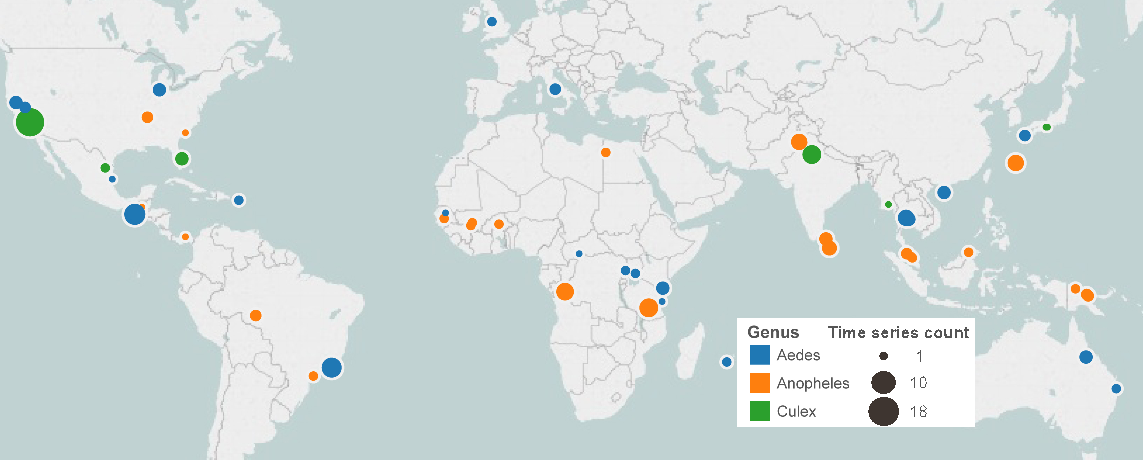
\includegraphics[width=1.25\textwidth]{./Figure_files/mrr_mapGenusCropped.pdf}}
	\caption{\textbf{The location and number of separate time-series for the MRR studies included in this analysis.} The area of each circle indicates the number of time-series at each study site. The colour shows the genus of the mosquitoes in each study.}
	\label{fig:mrr_lifetimes_map}
\end{figure}


\begin{table}[htbp]
	\centering
	\begin{tabular}{lc}
		\toprule
		\textbf{Data characteristic} & \textbf{Count} \\
		\midrule
		Species & 33 \\
		Genera & 3 \\
		\textit{Anopheles} & 94 \\
		\textit{Aedes} & 91 \\
		\textit{Culex} & 47 \\
		Female-only MRR & 179 \\
		Male-only MRR & 35 \\
		Mixed sex MRR & 18 \\
		Pre-release blood-feeding only MRR & 71 \\
		Pre-release sugar-feeding only MRR & 41 \\
		Pre-release both blood- and sugar-feeding MRR & 4 \\
		Pre-release neither blood- and sugar-feeding MRR & 116 \\
		MRR time-series & 232 \\
		\bottomrule
	\end{tabular}%
	\caption{\textbf{Summary of variables across all MRR time-series.} For the `Species' and `Genera' rows, the counts represent the number of distinct entries in the database; otherwise the counts represent the number of time series.}
	\label{tab:mrr_aggregateData}%
\end{table}%

\begin{table}[htbp]
	\centering
	\footnotesize
	\begin{adjustwidth}{-0.5in}{-0.5in}%
		\begin{tabularx}{1.25\textwidth}{l|ccccc}
			\toprule
			\textbf{Data characteristic} & \textbf{Min} & \textbf{Mean} & \textbf{Median} & \textbf{Max} & \textbf{Standard deviation} \\
			\midrule
			Study duration, days & 6.0   & 11.8  & 10.0  & 71.0    & 4.7 \\
			Number of days on which collections took place & 6.0   & 10.1  & 9.0   & 47    & 9.1 \\
			Number of separate release days & 1.0     & 1.9   & 1.0     & 23    & 3.0 \\
			Number released & 66    & 4,929  & 1,297  & 86,200 & 12,043 \\
			Number recaptured & 2     & 163   & 63    & 4,090  & 399 \\
			Recapture percentage & 0\% & 8.6\% & 5.2\% & 57.1\% & 10.04\% \\
			Age at release, days & 0   & 1.8   & 0   & 13    & 2.8 \\
			\bottomrule
		\end{tabularx}%
		\caption{\textbf{Summary of data from individual MRR time-series.}}
		\label{tab:mrr_IndividualData}%
	\end{adjustwidth}
\end{table}%

\begin{figure}[h]
	\centerline{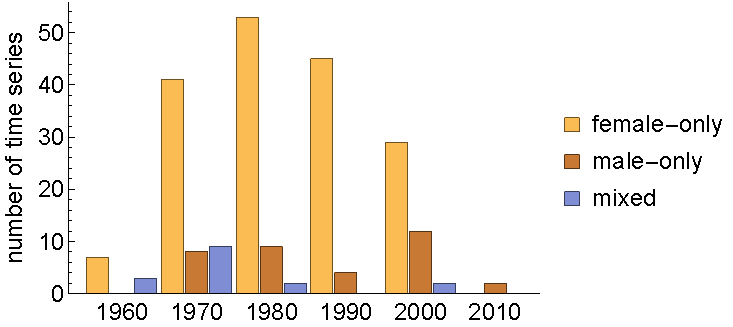
\includegraphics[width=1\textwidth]{./Figure_files/mrr_sexReleasesOverTime.pdf}}
	\caption{\textbf{The number of MRR time-series by date and sex of released mosquitoes.} The numbers represent by-decade totals of the 232 time-series we used in the main analysis.}
	\label{fig:mrr_sexReleasesOverTime}
\end{figure}


\subsection{Statistical model}\label{sec:mrr_statistical}
Data for a typical MRR experiment consists of a single release of $N_{R}$ marked mosquitoes followed by a series of marked mosquito recaptures on subsequent days (Fig. \ref{fig:mrr_exampleMRRSeries} shows three such example series). We model the number $y(t)$ of marked mosquitoes recaptured on day $t$ using a negative binomial sampling model,
%
\begin{equation}\label{eq:NB}
y(t) \sim \text{NB}\left((N_{R} - Y(t-1)) S(t) \psi, \kappa\right),
\end{equation}
%
where $Y(t-1)$ is the cumulative number of mosquitoes caught on all days before $t$, $S(t)$ is the probability that an individual mosquito survives and remains in the study area until time $t$, $\psi$ is the daily recapture probability for an individual mosquito which is assumed constant through time, and $\kappa$ is the time-independent shape parameter of the negative binomial distribution that controls the extent of variance in recapture rate likely due mostly to environmental heterogeneity. We chose a parameterisation of the negative binomial such that its mean is given by $\mu(t) = (N_{R} - Y(t-1)) S(t) \psi$, and its variance by $\sigma(t)^2 = \mu(t) + \frac{\mu(t)^2}{\kappa}$. 

For some MRR experiments, there were a number of releases ($q\geq 2$) of marked mosquitoes throughout the duration of the study. In contrast to single releases, with multiple releases over time, it is not in general possible to determine the particular release to which a recaptured mosquito belongs. To avoid the complication of directly inferring this quantity, we choose to represent previous recaptures probabilistically. This results in a slightly different mean to that of the single release model,
%
\begin{equation}
\mu(t) = N_{Released}(1-\psi)^{t-1} S(t) \psi,
\end{equation}
%
where the factor of $(1-\psi)^{t-1}$ represents the probability that a mosquito is \textit{not} recaptured on a previous day. Where experiments consisted of two or more releases occurring at distinct points in time we assumed that recaptures of individual mosquitoes from either batch were independent of one another, although with the same sampling parameters ($\psi$ and $\kappa$). This results in an overall mean composed of the sum of those from all $q$ releases,
%
\begin{equation}
\mu(t) = \mu_1(t) + ... + \mu_q(t).
\end{equation}
%

\begin{figure}[h]
	\centerline{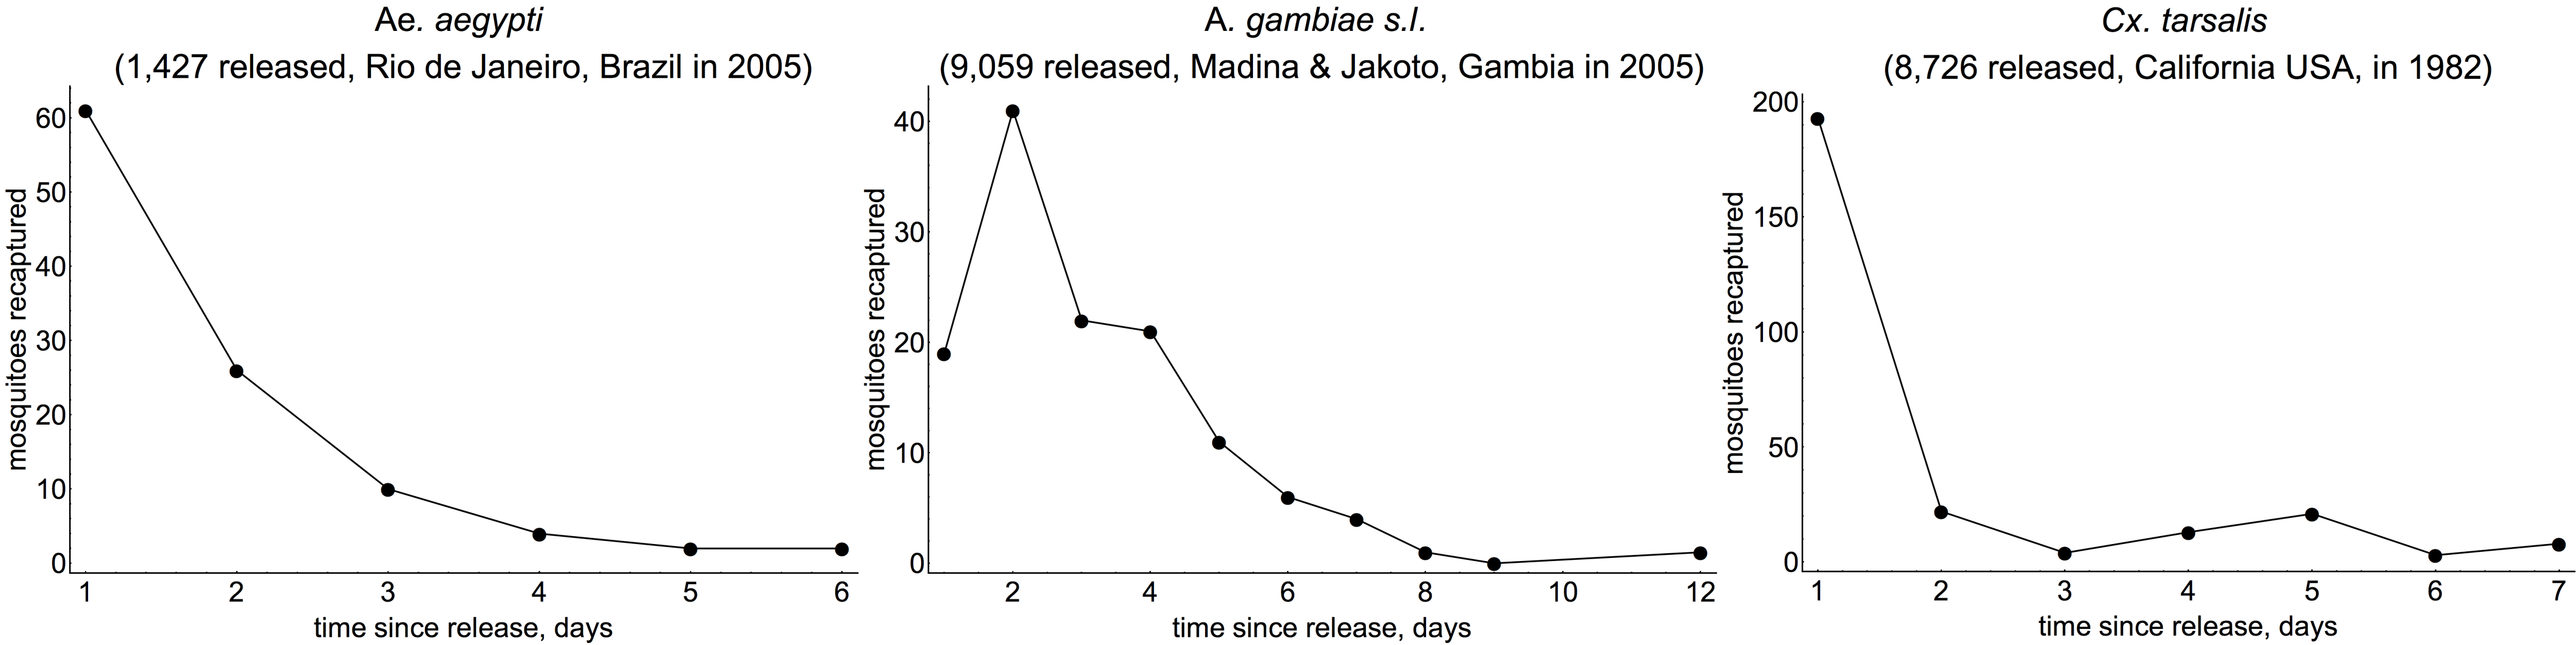
\includegraphics[width=1.25\textwidth]{./Figure_files/mrr_exampleMRRSeries.pdf}}
	\caption{\textbf{Example MRR time-series for three different studies from the \cite{guerra2014global} database.} In all the above experiments there was a single release of a batch of marked mosquitoes.}
	\label{fig:mrr_exampleMRRSeries}
\end{figure}

The simplest assumption is that death and dispersal rates are independent of mosquito age, giving an exponential `survival' function,
%
\begin{equation}
S(t) = e^{-\lambda t},
\end{equation}
%
where $\lambda$ is the sum of the rates of death and dispersal from the study area. To estimate the lifespan of mosquitoes we use this model, partly because of the limited evidence we determine in favour of senescence (Figs. \ref{fig:mrr_elpd} and \ref{fig:dissection_elpd}).

We assume that the number of mosquitoes recaptured on one day is independent of the number recaptured on any other day, apart from their joint dependence on $\lambda$, $\psi$ and $\kappa$. This results in a likelihood of the data of the form,
%
\begin{equation}
\mathcal{L}(y(t_1),y(t_2),...,y(t_R)|\lambda,\psi,\kappa) = \prod\limits_{i=1}^{R} p(y(t_i)|\psi,\lambda,\kappa),
\end{equation}
%
where $R$ is the number of individual days where collections took place, and $p(y(t_i)|\psi,\lambda,\kappa)$ is the probability of recapturing $y(t_i)$ mosquitoes on day $t_i$ determined from a negative binomial distribution with parameters $\mu = e^{-\lambda t} \psi$, and $\kappa$.

\subsection{Individual time-series estimates}\label{sec:MRR_individual_analysis}
We first treat each time-series separately, and estimate individual $(\lambda,\psi,\kappa)$ parameters of the statistical model (described in the previous section) for each time-series. To use a Bayesian methodology we must specify priors on this set of parameters. Here we choose to specify independent priors on each parameter of the form: $\lambda\sim \mathcal{N}(-2.32,1)$, $\psi\sim \text{exp}(50)$ (with $\psi$ constrained to be less than 0.1, a threshold below which the majority of daily recapture probabilities in the data are observed) and $\kappa\sim \textnormal{log-normal}(2,1)$. This prior on the rate parameter of the exponential distribution ($\lambda$) corresponds to a wide range of possible lifespans (Fig. \ref{fig:mrr_individualTimeSeries_priors}A), with a mean of 10 days. It was necessary to use an informative prior on $\psi$ to bound it to sensible values and to prevent the correlation of estimates with $\lambda$ leading to unreasonably short estimates of $\lambda$; the prior on $\kappa$ is fairly uninformative and allows a wide range of values (Fig. \ref{fig:mrr_individualTimeSeries_priors}B,C). 


\begin{figure}[h]
	\centerline{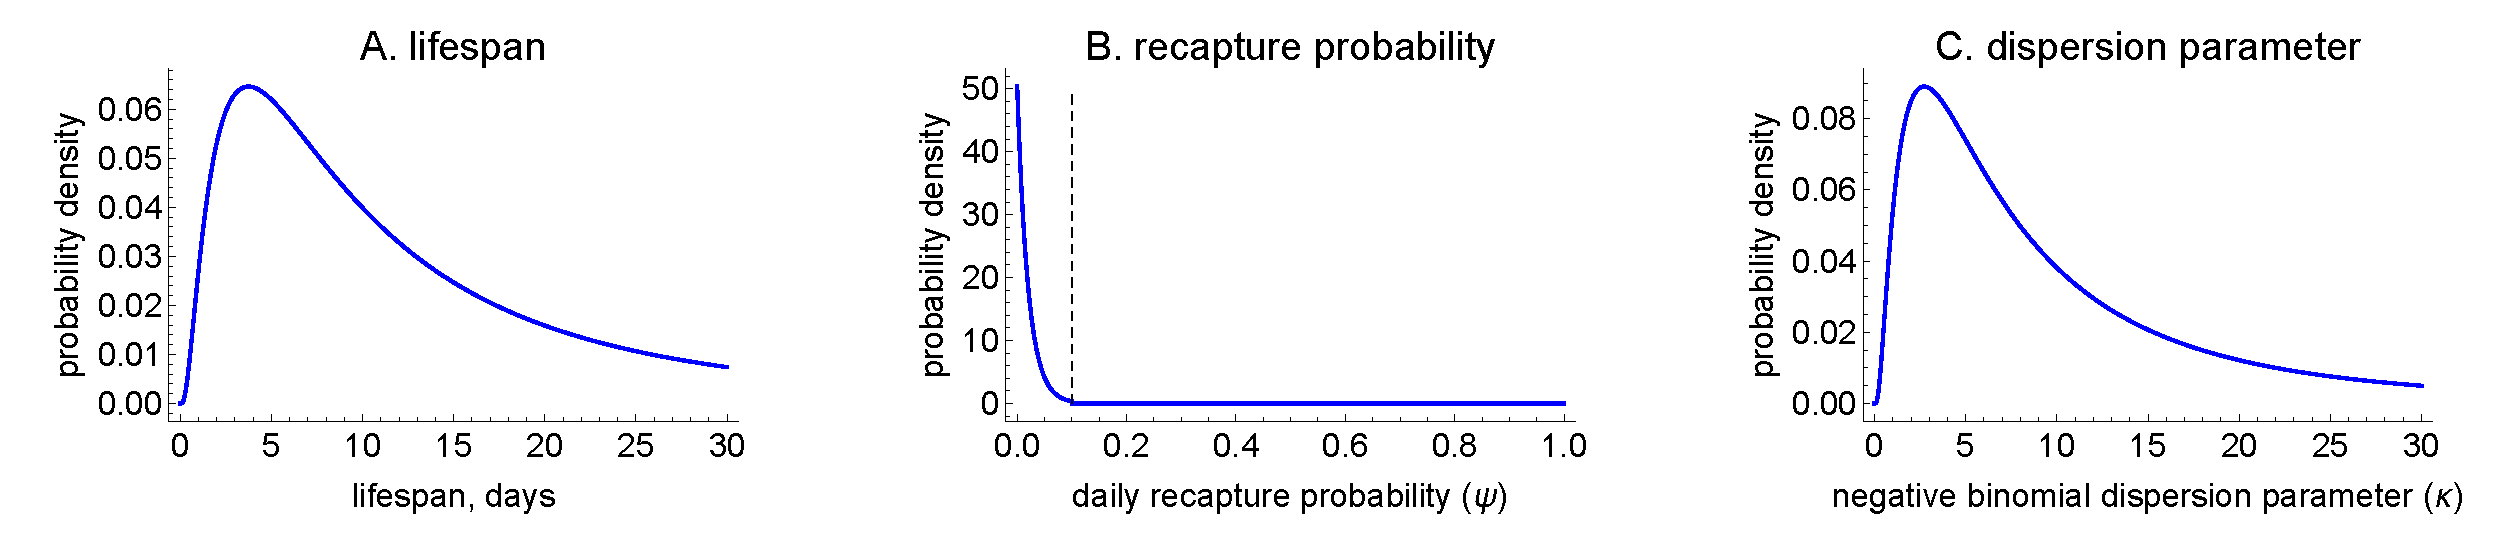
\includegraphics[width=1.25\textwidth]{./Figure_files/mrr_individualTimeSeries_priors.pdf}}
	\caption{\textbf{The prior probability distributions used for lifespan (A), recapture probability (B) and dispersal parameter (C) in the individual time-series analysis for the MRR studies.} Note: the prior for the recapture probability was truncated at $\psi=0.1$ since most MRR day one recapture fractions were significantly below this threshold.}
	\label{fig:mrr_individualTimeSeries_priors}
\end{figure}

\subsection{Estimating lifespan at the species, genus and overall groupings}\label{sec:MRR_hierarchical}
We synthesise information from across all MRR experiments to produce more robust estimates of mosquito lifespan than can be obtained from considering the individual time-series separately. However there exists considerable heterogeneity across the experiments. This heterogeneity has two sources. There is that arising from variability in experimental methodology. There is also variability from actual differences in lifespan across the different mosquito cohorts; for example due to genetic differences between mosquito populations or due to climatic differences. Because of this heterogeneity we use a Bayesian hierarchical model which is akin to a `random effects' model in classical statistics. This type of model assumes that there is random variation in parameters at the individual time-series level, although each of the parameters is drawn from a common `population-level' distribution. In our case we separately estimate three different model groupings where the population-level distributions correspond to the species, genus and overall (across all studies) levels respectively (Fig. \ref{fig:mrr_methodDiagramHierarchy}). This allows us to estimate average mosquito lifespan for a given species or genus, or alternatively across all time-series, by independent sampling from the posterior predictive distribution from which the individual $\lambda_i$ are drawn.


\begin{figure}[h]
	\centerline{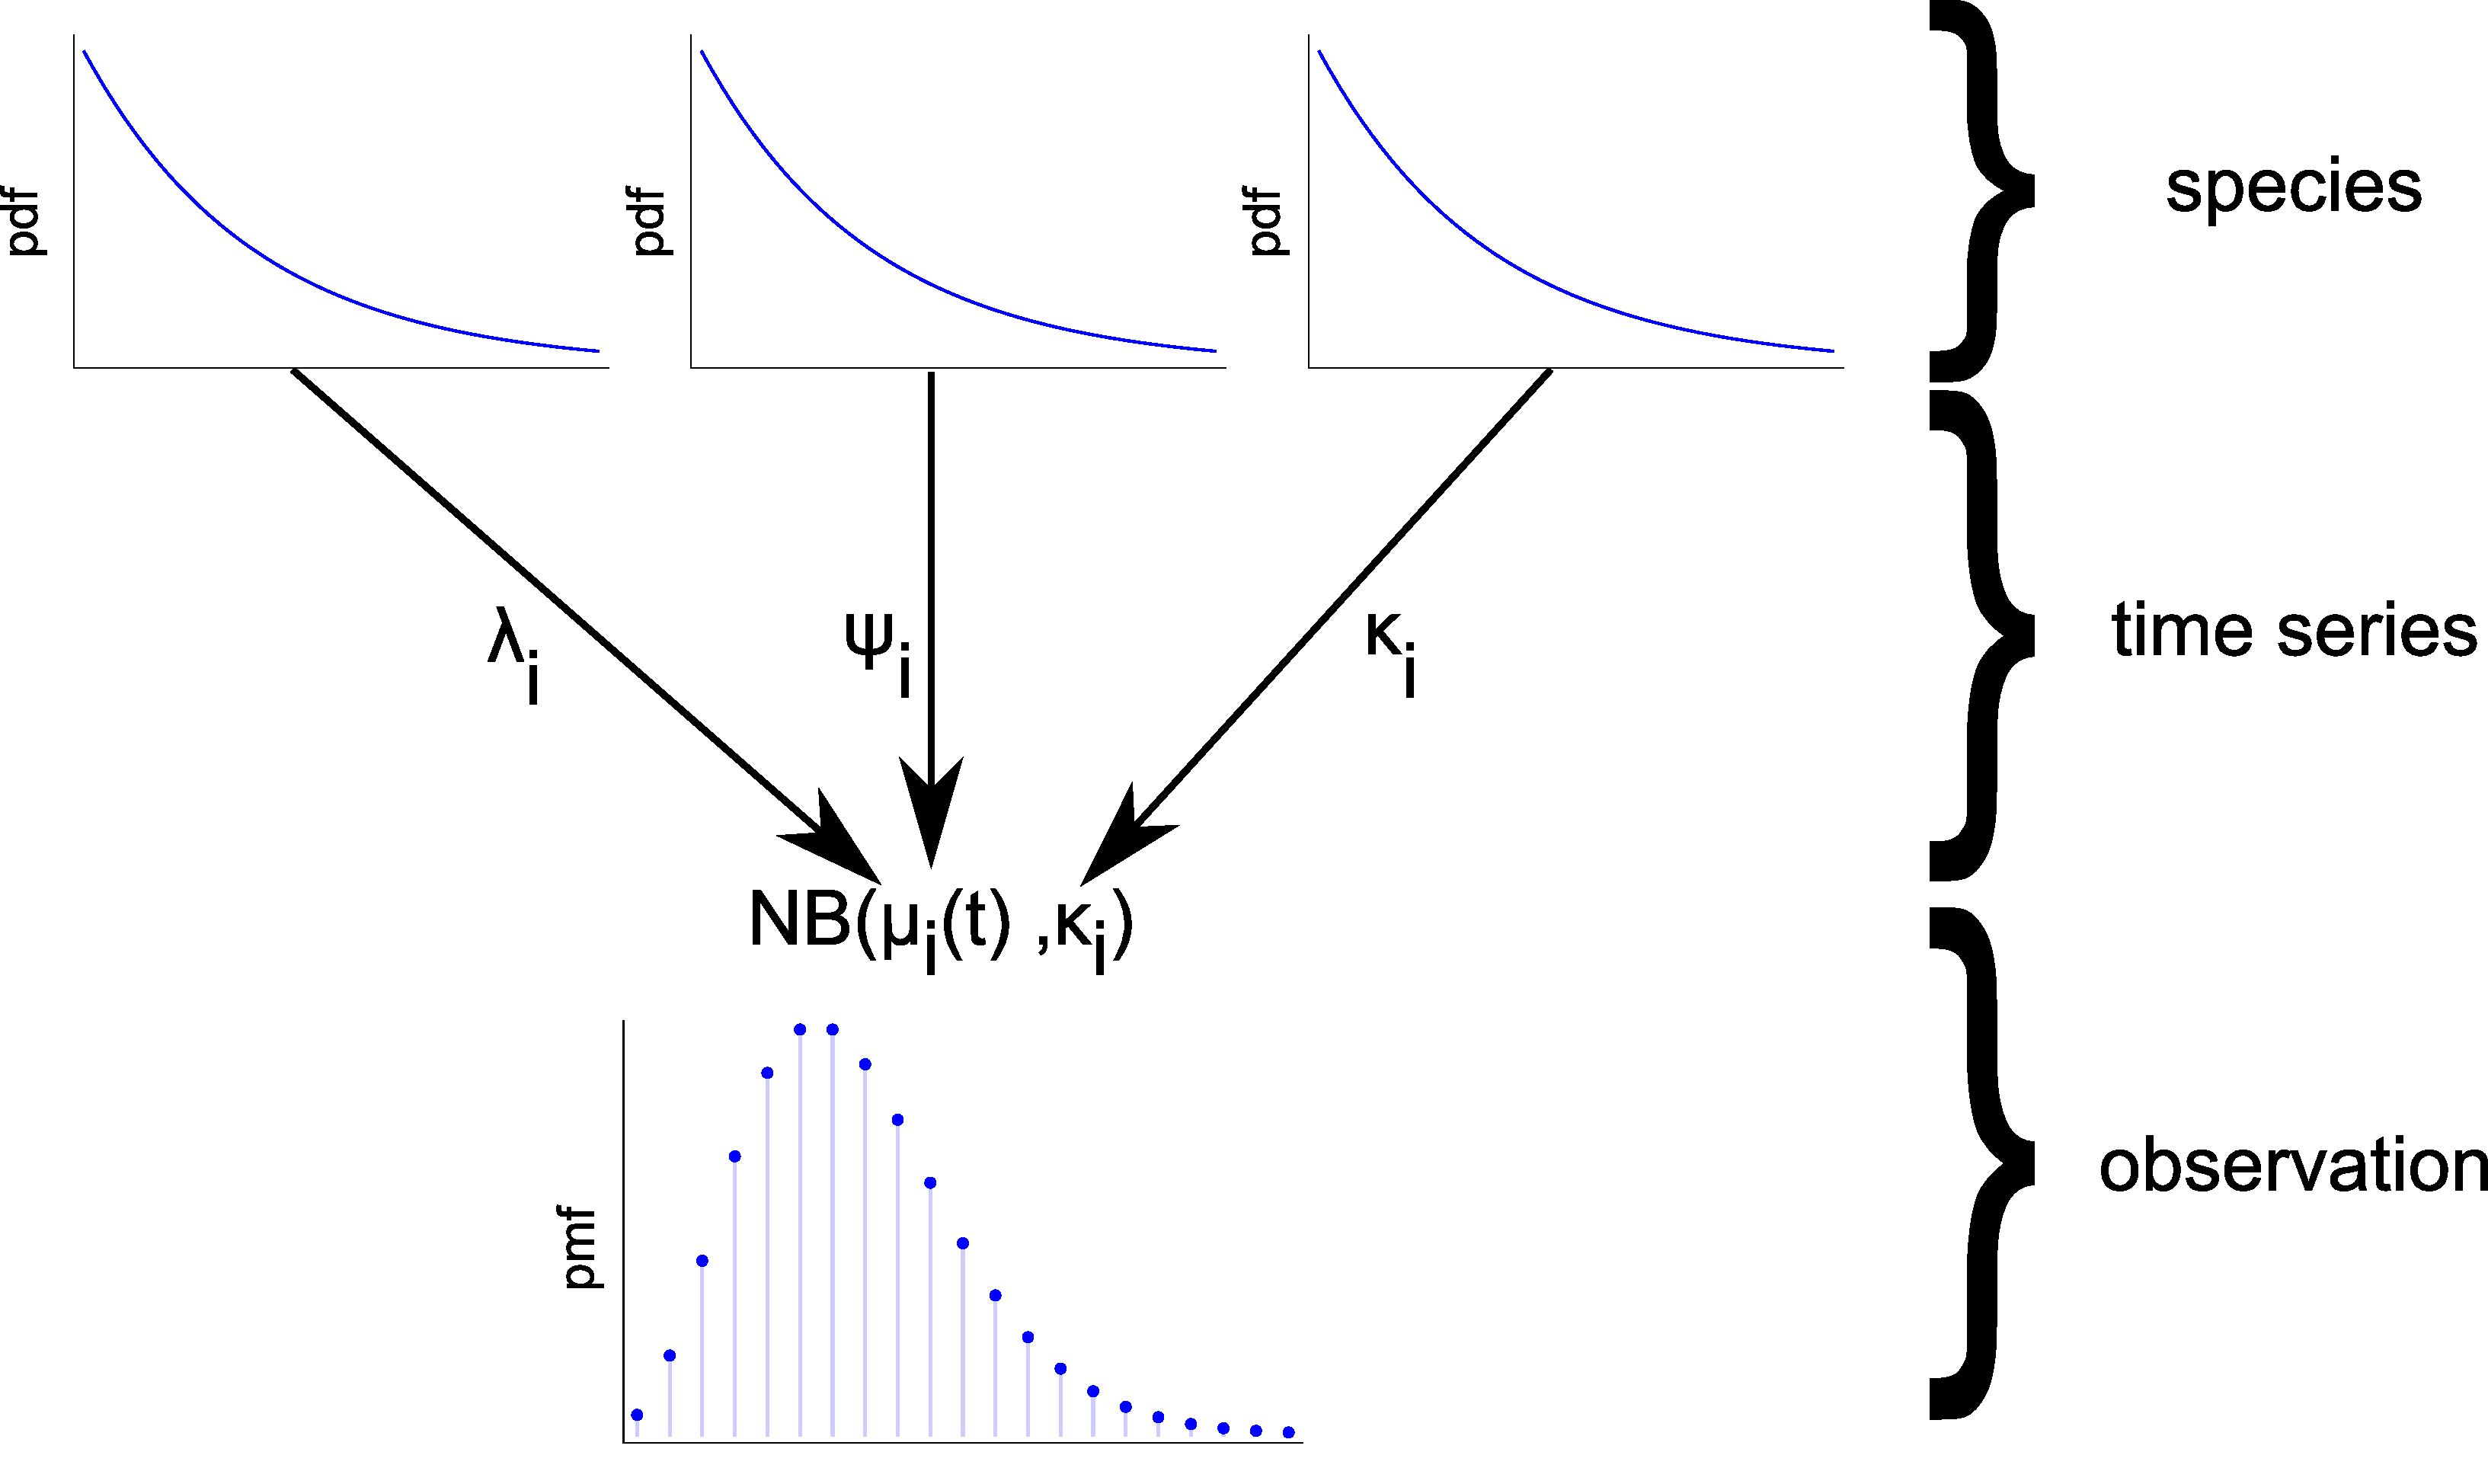
\includegraphics[width=1\textwidth]{./Figure_files/mrr_methodDiagramHierarchy.pdf}}
	\caption{\textbf{A representation of the hierarchical Bayesian model, for the constant mortality model case when considering the species-level grouping.} Here `pdf' indicates `probability density function', and $\lambda_i$, $\psi_i$, and $\kappa_i$ represent the force of mortality for the exponential distribution, daily recapture probability and over-dispersion parameter of the negative binomial distribution for time-series $i$ in the dataset; $\mu_i(t)= \psi_i e^{-\lambda_i t}$ is the mean number of mosquitoes recaptured on day $t$.}
	\label{fig:mrr_methodDiagramHierarchy}
\end{figure}

Whilst we assume that the variation in mosquito mortality across experiments is random in nature, we recognise that there may exist systematic sources of variation that we do not include in our model. To account for this potential source of bias we examined how the individual estimates of lifespan correlated with experimental covariates (trapping method and number or density of traps). The data on trapping method in the Guerra et al., (2014) database is less reliable than other data entries because published MRR studies may use multiple trapping methods and typically do not disaggregate captures by method. When we examined the correlation of trapping method with lifespan estimates, however, we did not find systematic variation by method (data not shown). We determined a positive correlation between trapping density and lifespan estimates (Fig. \ref{fig:mrr_lifeSpanVsTrapDensity}), which indicates the impact of mosquito dispersal on estimated lifespan.

A Bayesian framework requires that we incorporate our pre-analysis beliefs into our estimates through the use of priors for all parameters in a particular model. In our hierarchical model we are required to specify prior distributions at two levels of the analysis. The first of these links the individual time-series estimates with the overarching group-level distributions. The parameters of these group-level distributions are then set prior distributions (Fig. \ref{fig:mrr_methodDiagramHierarchy}). As an example, we suppose that the rate parameter $\lambda_i$ of our exponential survival model in experiment $i$ is given by:
%
\begin{align}
\lambda_i = \text{exp}(&c_i + \delta^m_{\text{genus}[i]} \text{sex}^{\text{m}}_i + \delta^{\text{mix}}_{\text{genus}[i]} \text{sex}^{\text{mix}}_i +\\  & \delta^{\text{sugar}}_{\text{genus}[i]} \text{sugar}_i +  \delta^{\text{blood}}_{\text{genus}[i]} \text{blood}_i),
\end{align}
%
where $\delta^m_{\text{genus}[i]}$ measures a genus-specific effect of male-only releases ($\text{sex}^{\text{m}}_i=1$) versus female-only ($\text{sex}^{\text{m}}_i=0$); $\delta^{\text{mix}}_{\text{genus}[i]}$ is the analogous effect for mixed releases versus female-only; $\delta^{\text{sugar}}_{\text{genus}[i]}$ is the analogous effect for mosquitoes that were sugar-fed prior to release versus those that were not fed; and $\delta^{\text{blood}}_{\text{genus}[i]}$ is the analogous effect for mosquitoes that were blood-fed prior to release versus those that were not fed. The parameter $c_i$ is modelled hierarchically, being drawn from a group-level distribution assumed to be normal,
%
\begin{equation}
c_i \sim  \mathcal{N}(\mu_\lambda,\sigma)
\end{equation}
%
We then specify priors on these group-level parameters, $\mu_\lambda \sim \mathcal{N}(-2.32,1)$ and $\sigma \sim \textnormal{log-normal}(-3,1)$. On all $\delta$ parameters, except $\delta^{\text{mix}}_{\text{genus}[i]}$, we specify standard normal priors. We specify a uniform prior on $\delta^{\text{mix}}_{\text{genus}[i]}\sim U(0,\delta^m_{\text{genus}[i]})$ so that the effect of mixed releases lies between the female-only release effect (0) and the male-only release effect ($\delta^m_{\text{genus}[i]}$). 

The relatively complex nature of priors in hierarchical models make it important to determine their influence on inferences. We chose the above -- somewhat uninformative -- priors to allow a range of mosquito lifespans in order to minimise their effect on the estimates we report (Fig. \ref{fig:mrr_meanLifespanPrior}). We also chose to set hierarchical priors on the remaining parameters in our models -- $\psi$ the probability of daily recapture, and $\kappa$ the `over-dispersion' parameter of a negative binomial distribution. For $\psi$ we chose an informative prior that placed all probability mass $\psi\leq 10\%$, since in most experiments the fraction of mosquitoes captured was significantly below this value. For $\kappa$ we chose a fairly wide prior that had most of its probability mass below $\kappa=20$ (Fig. \ref{fig:mrr_PsiKappaPriors}). In all cases the hierarchical priors were chosen to have similar implications on lifespan, recapture probability and over-dispersion at the individual time-series level as for the non-hierarchical analysis described previously.

\begin{figure}[h]
	\centerline{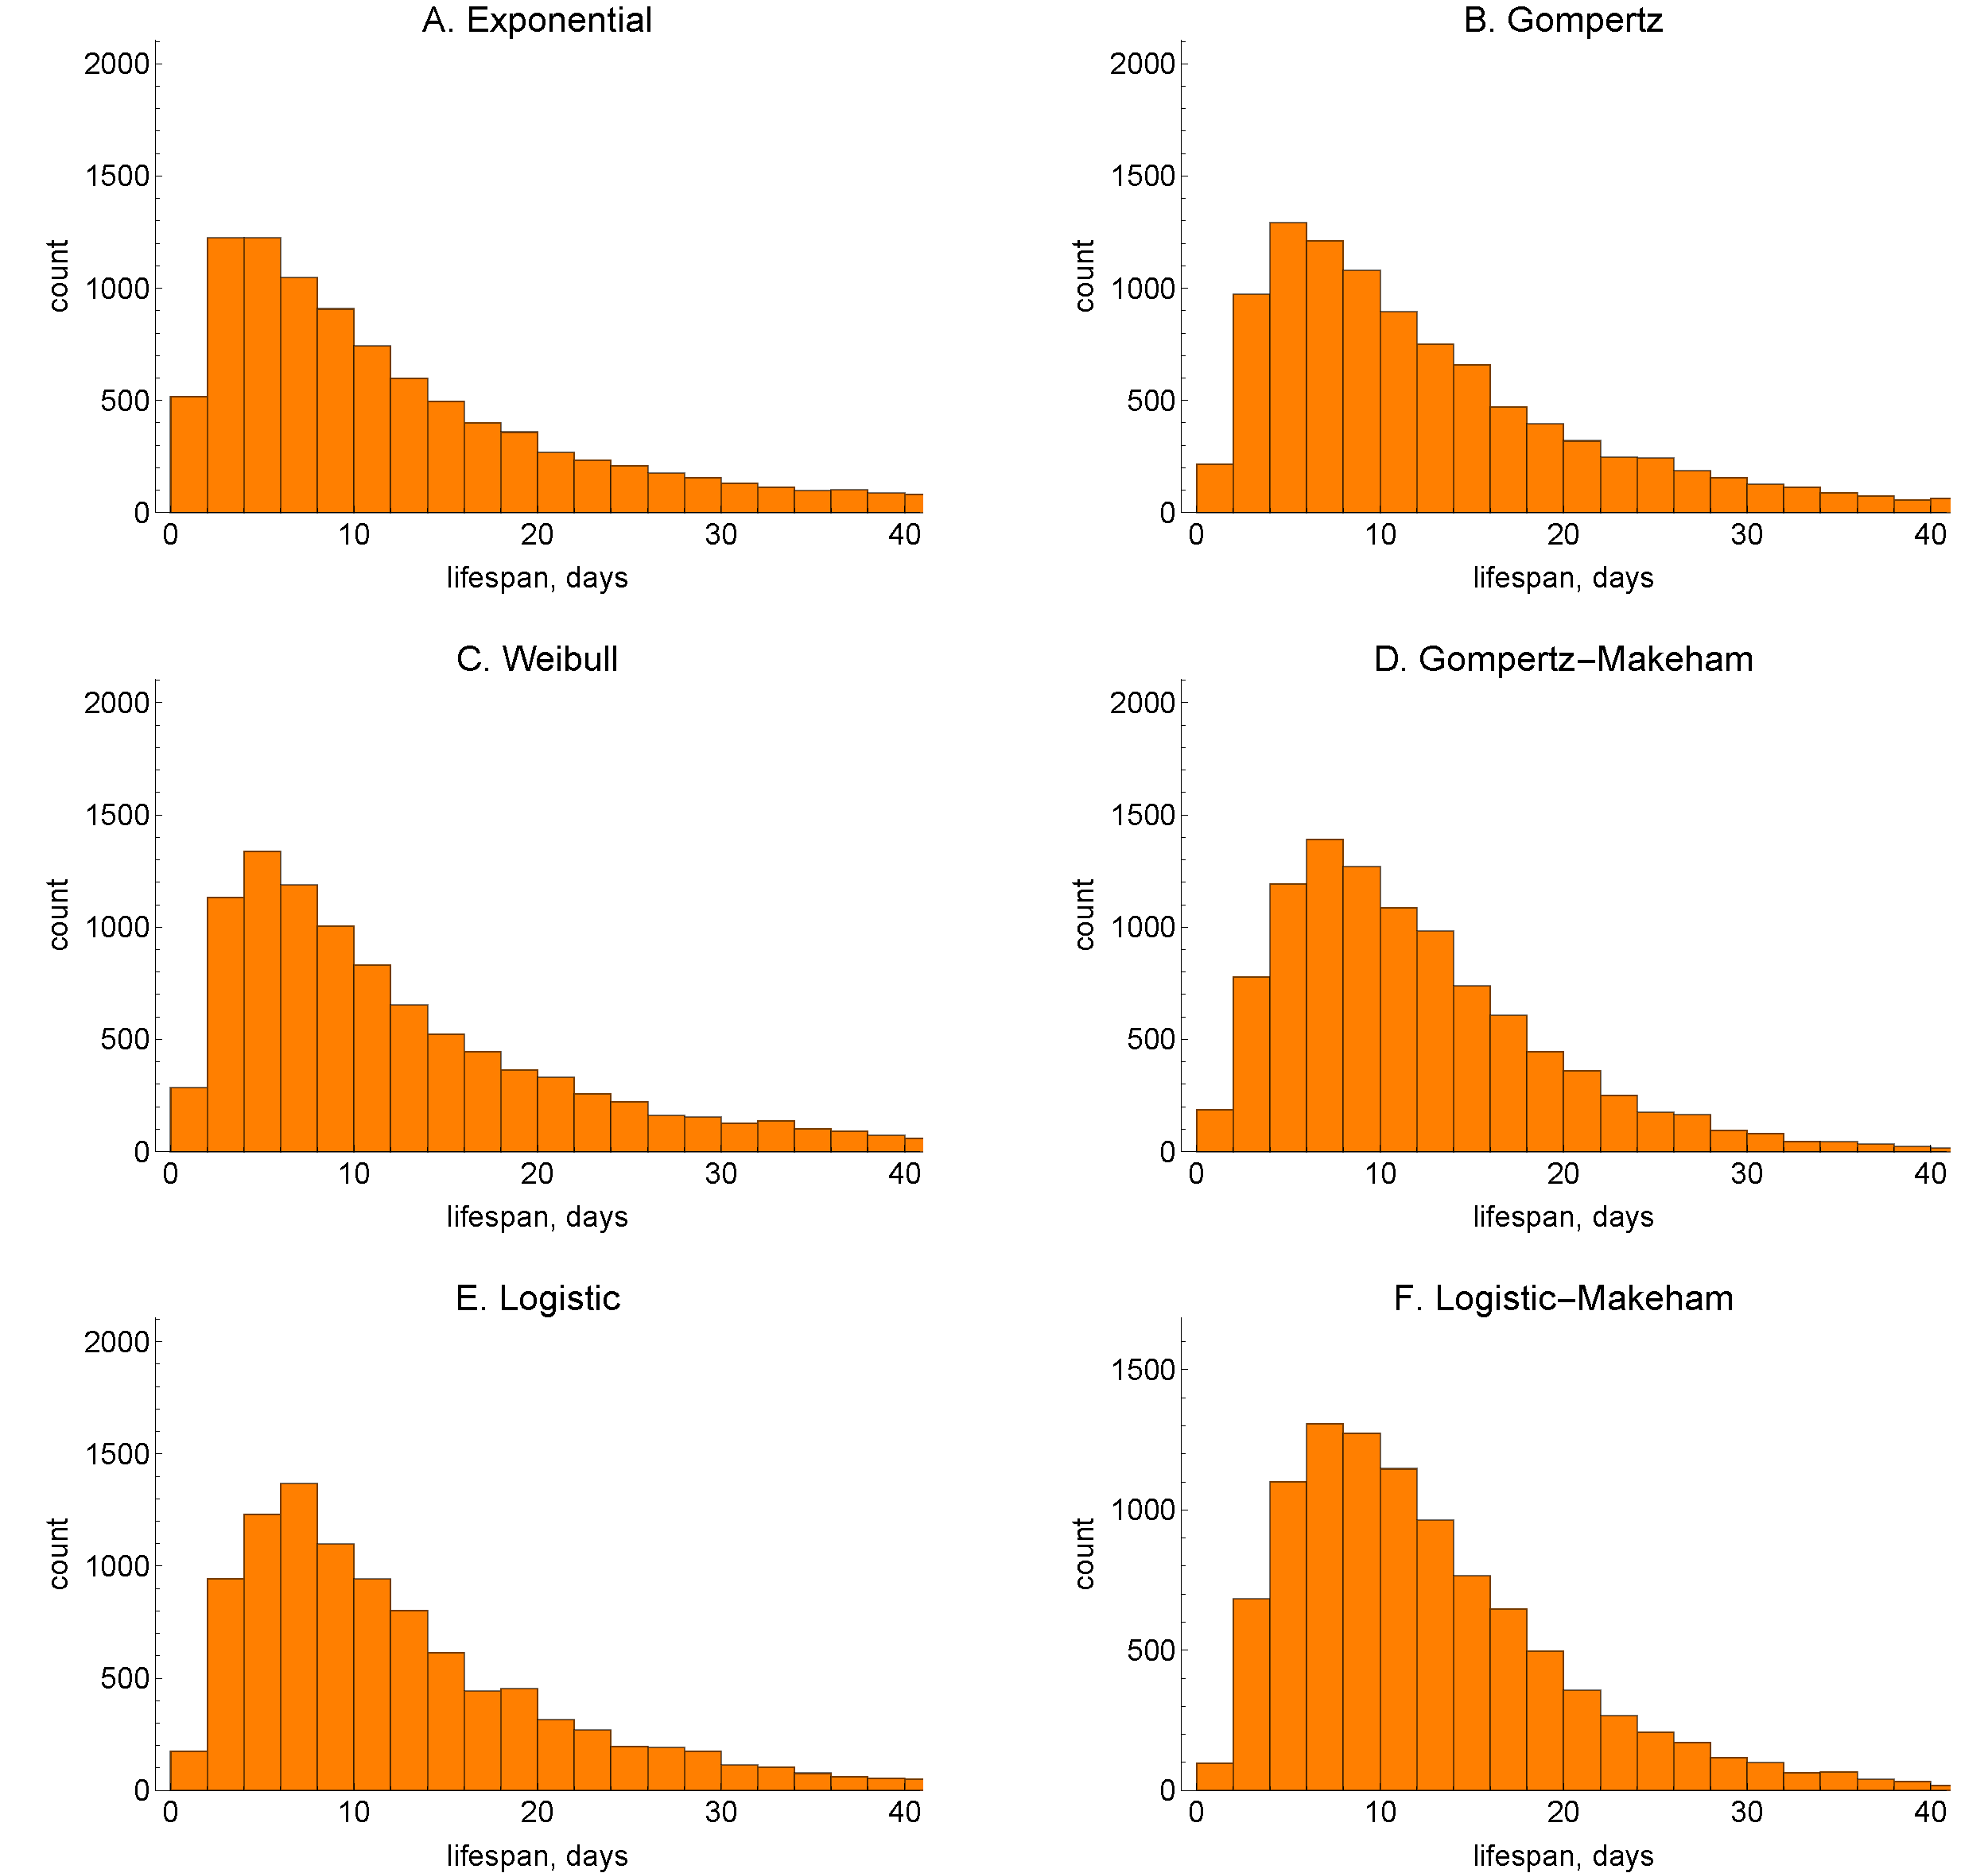
\includegraphics[width=1\textwidth]{./Figure_files/mrr_lifespan_priors.pdf}}
	\caption{\textbf{Samples from the prior predictive distribution of mean lifespan across the six models of mosquito mortality introduced in Table \ref{tab:mrr_survivalDescription}.} In all cases 10,000 samples were generated using the priors indicated in Table \ref{tab:mrr_priors}, resulting in distributions with a mean close to 10 days.}
	\label{fig:mrr_meanLifespanPrior}
\end{figure}

\begin{figure}[h]
	\centerline{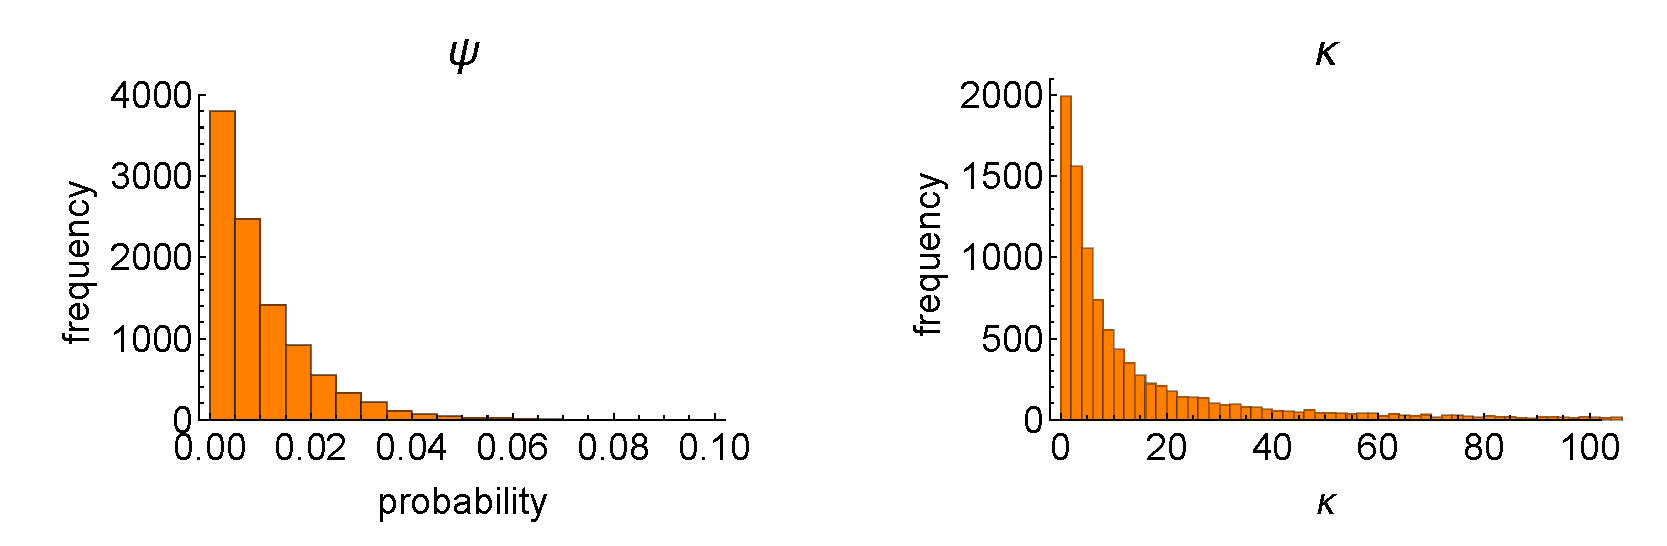
\includegraphics[width=1\textwidth]{./Figure_files/mrr_priors_PsiKappa.pdf}}
	\caption{\textbf{Samples from the priors for daily recapture probability ($\psi$) and over-dispersion parameter ($\kappa$).} In both panels, 10,000 samples were generated using the following hierarchical priors: for the individual time series parameters, $\psi_i \sim \text{exp}(r)$ (with $\psi$ constrained to be less than 0.1 - encompassing the upper limit of day one recapture fractions observed in most data series) and $\kappa_i \sim \text{exp}(p)$; for the top-level parameters: $r\sim \text{gamma}(100, 2)$ and $p\sim \text{log-normal}(1.5, 1)$.}\label{fig:mrr_PsiKappaPriors}
\end{figure}

\subsection{Testing for age-dependent mortality in wild mosquitoes}\label{sec:mrr_age_dependence}
Previous work has found evidence of age-dependent mortality in lab populations \citep{styer2007mosquitoes,dawes2009anopheles}, and less-commonly in wild mosquitoes \citep{clements1981analysis}. Furthermore, recent modelling work has examined the implications of departures from a constant risk of mortality \citep{styer2007mosquitoes,hancock2009age,novoseltsev2012age}. To determine whether senescence occurs in wild mosquitoes we re-estimate our model using survival functions, $S(t)$, that allow for a rate of mortality that can vary with age. Specifically, we re-estimate our model using five other models that were previously used in the literature (see Table \ref{tab:mrr_survivalDescription} for a description of these). Each of these models makes different assumptions about how the rate of death and dispersal varies with age, but all can be represented by a general form,
%
\begin{equation}\label{eq:survivalInt}
S(t) = e^{-\int\limits_{0}^{t}\lambda(\tau) \mathrm{d}\tau}.
\end{equation}
%
where we constrain the parameters of our models to preclude the possibility of a hazard that decreases with age ($\frac{\mathrm{d}\lambda(t)}{\mathrm{d}t} \geq 0$). Whilst this could occur if older mosquitoes disperse less than younger mosquitoes, it is unlikely this would outweigh any declines in survival associated with old age.

The parameters of the survival function of each model were assigned hierarchical priors that allowed considerable variation in mosquito lifespan (see Fig. \ref{fig:mrr_meanLifespanPrior}). Otherwise the statistical model we used remained the same as for the constant mortality case. In testing for age-dependent mortality, we did not account for sex or pre-release feeding effects due to the complexity of including these elements in more complex survival models.

\begin{table}
	\scriptsize
	\noindent\makebox[\textwidth]{%
		\begin{tabularx}{1.35\textwidth}{c|cXcX}
			\textbf{Survival function} & \textbf{Hazard rate} & \textbf{Interpretation} & \textbf{Mean time spent in study area, }\textbf{$\overline{T}$} & \textbf{Papers assuming this function} \\
			\midrule
			Exponential & $\lambda$ & Constant mortality risk & $\frac{1}{\lambda}$ & \cite{ross1910prevention}; \cite{anderson1992infectious}; \cite{smith2004statics} \\
			\midrule
			Gompertz &  $\alpha e^{\beta t}$     & Mortality increases with age at an ever-increasing rate &  $\frac{e^{\frac{\alpha}{\beta}} \Gamma(0,\frac{\alpha}{\beta})}{\beta}$    & \cite{clements1981analysis}; \cite{styer2007mosquitoes};\cite{novoseltsev2012age} \\
			\midrule
			Weibull &  $\alpha t^\beta$; $\;\beta\geq 1$     &  Mortality increases with age at an ever-increasing rate     &   $\alpha^{-\frac{1}{\beta}} \Gamma(1+\frac{1}{\beta})$    & \cite{hancock2009age}; and \cite{carey2001insect} considering general insect demography \\
			\midrule
			Gompertz-Makeham &  $\alpha e^{\beta t} + c$      &  Two additive mortality risks: one that increases with age, and another that is age-independent  &  No simple analytic form     & \cite{styer2007mosquitoes} \\
			\midrule
			Logistic & $\frac{\alpha e^{\beta t}}{1+\frac{\alpha s}{b}\left(e^{b t} - 1\right)}$   & Mortality risk increases with age, although at a declining rate  & No simple analytic form   & \cite{styer2007mosquitoes}; \cite{novoseltsev2012age} \\
			\midrule
			Logistic-Makeham &   $\frac{\alpha e^{\beta t}}{1+\frac{\alpha s}{b}\left(e^{b t} - 1\right)} + c$    & Two separate additive mortality risks: an age-dependent risk of the same form as the logistic model, and a constant hazard  &  No simple analytic form  & \cite{styer2007mosquitoes}; \cite{bellan2010importance} \\
			\bottomrule
	\end{tabularx}}
	\caption{\textbf{A description of the survival functions used in this study, arranged in rough order of model complexity (simple-complex from top-bottom.)} All parameters are defined to be non-negative. $\Gamma(\theta)$ and $\Gamma(\theta_1,\theta_2)$ refer to the Euler gamma function, and incomplete gamma function respectively. The `mean time spent in study area' is an estimate of the combined effects of mosquito mortality and dispersal from the area of the study where collections take place, since our data does not provide spatially-resolved data.}\label{tab:mrr_survivalDescription}
\end{table}

\begin{table}
	\footnotesize
	\noindent\makebox[\textwidth]{%
		\begin{tabularx}{1.2\textwidth}{l|c|X}
			\textbf{Survival function} & \textbf{time-series-level priors} & \textbf{Group-level priors}\\
			\midrule
			Exponential & $c\sim \mathcal{N}(\mu_\lambda,\sigma)$ &$\mu_\lambda \sim N(-2.32,1)\text{,}\; \sigma\sim \textnormal{log-normal}(-3,1)$\\
			\midrule
			Gompertz & $\alpha,\beta\sim$ log-normal$(\mu_{\alpha|\beta},0.2)$ &$\mu_\alpha\sim N(-3,1)\text{,}\; \mu_\beta\sim N(-3,1.1)$\\
			\midrule
			Weibull & $\alpha,(\beta-1)\sim$  log-normal$(\mu_{\alpha|\beta},0.2)$ &$\mu_\alpha\sim N(-4.8,1.75)\text{,}\; \mu_\beta\sim N(-4,2)$\\
			\midrule
			Gompertz-Makeham & $\alpha,\beta,c\sim$ log-normal$(\mu_{\alpha|\beta|c},0.2)$ &$\mu_\alpha\sim N(-3,1)\text{,}\; \mu_\beta\sim N(-3,0.5)\text{,}\; \mu_c\sim N(-4.5,0.5)$\\
			\midrule
			Logistic & $\alpha,\beta,s\sim$  log-normal$(\mu_{\alpha|\beta|s},0.2)$ &$\mu_\alpha\sim N(-2.8,1)\text{,}\; \mu_\beta\sim N(-3,1)\text{,}\; \mu_s\sim N(-3,1)$\\
			\midrule
			Logistic-Makeham & $\alpha,\beta,s,c\sim$ log-normal$(\mu_{\alpha|\beta|s|c},0.2)$ &$\mu_\alpha\sim N(-3.2,1)\text{,}\; \mu_\beta\sim N(-3.2,1)\text{,}\; \mu_s\sim N(-3,0.5)\text{,}\; \mu_c\sim N(-4,0.5)$\\
			\bottomrule
	\end{tabularx}}\caption{\textbf{The priors used on parameters of each different survival model.} For the exponential model the `group-level' priors were the same for the genus and `overall' models that were also estimated. The exponential model was the only model that was simple enough to allow the scale parameter of the log-normal ($\sigma$) to be estimated by the data. The notation $\alpha,\beta\sim \text{log-normal}(\mu_{\alpha|\beta},0.2)$ means that $\alpha$ and $\beta$ were assigned independent log-normal priors with location parameters $\mu_\alpha$ and $\mu_\beta$ respectively, and a scale parameter of 0.2 in both cases.}\label{tab:mrr_priors}
\end{table}


\subsection{Model estimation by MCMC}\label{sec:mrr_MCMC}
The likelihood and priors we use result in posterior distributions whose analytic form cannot be calculated with existent computational methods. Instead we use Markov Chain Monte Carlo (MCMC) methods to sample from each posterior distribution. We used \textit{Stan} software \citep{carpenter2016stan} that implements an efficient MCMC algorithm known as NUTS \citep{hoffman2014no}.

To judge convergence of the sampling algorithm to the posterior density, we calculated $\hat{R}$ across all Markov chains -- a ratio that compares the between-chain variation to that within each chain that is commonly used to measure convergence in MCMC \citep{gelman1992inference}. For each class of model, we used the following MCMC parameters,
%
\begin{itemize}
	\item Individual lifespan models (Section \ref{sec:MRR_individual_analysis}): 12 independent chains with 1000 iterations per chain,
	\item Hierarchical lifespan estimates (Section \ref{sec:MRR_hierarchical}): 12 independent chains with 15,000 iterations per chain,
	\item Age-dependent analysis (Section \ref{sec:mrr_age_dependence}): 12 independent chains with 3000 iterations per chain.
\end{itemize}

In all cases, we discarded the first half of these iterations as warm-up \citep{gelman2014bayesian}. At the end of all runs for lifespan estimation, $\hat{R}<1.1$ for all model parameters. For the age-dependent cases, there remained a handful of parameters where $\hat{R}>1.1$ after running simulations for 3000 iterations but this did not affect our inferences, since repeated runs demonstrated the same pattern. We also ensured that across each MCMC run the number of divergent iterations (that can bias the MCMC away from the true posterior density) was minimal. In the majority of cases, the number of divergent iterations was far fewer than 1\% of the total number of samples.

The Stan scripts for the lifespan estimation (i.e. those using an exponential survival model) for the MRR analyses are provided below. The script for the individual time series analysis (Section \ref{sec:MRR_individual_analysis}):

\begin{minted}{stan}
data {
// Single release parameters
int<lower=0> N; // number of observations
int<lower=0> K; // number of groups
int Y[N]; // observations for the releases
int S[K]; // time series lengths
vector[N] t; // time observations (days) 
int Pos[K]; // starting position of each dataset

// Multiple release parameters
int RelFreq[K]; // frequency of releases in each study
// starting position of releases in each study
// in RelNumber
int PosRel[K];
int<lower=0> NReleases; // total number of releases
// numbers released in each study
vector[NReleases] RelNumber;
// time of each release in each study
vector[NReleases] RelTime;

real Age[K];
} 

parameters {
real<lower=0.3, upper=20> kappa[K];
real<lower=0> cDecay[K];
real<lower=0, upper=1> psi[K];
} 

model {
// Likelihood
for (i in 1:K) {
real lambda[S[i]];

if (RelFreq[i]< 2) // Single release
{
   real numberCaught;
   numberCaught = 0;	
   for (j in 1:S[i])
   {
     lambda[j]= (psi[i] *
                (RelNumber[PosRel[i]] - numberCaught) *
                exp(-cDecay[i] * (t[Pos[i] + j - 1] + Age[i])));
     //1e-5 to prevent loc=0
     Y[Pos[i] + j - 1] ~ neg_binomial_2(
        		lambda[j] + 1e-5, kappa[i]); 
     numberCaught = numberCaught + Y[Pos[i] + j - 1];
   }
} else // Multiple release
  {
    for (j in 1:S[i])
    {
      real lambdaTemp;			
      lambdaTemp = 0;
      for (kk in 1:RelFreq[i])
      {
        if (t[Pos[i] + j - 1]> RelTime[PosRel[i]+kk-1])
        {
           lambdaTemp = (
                   lambdaTemp +
                   RelNumber[PosRel[i] + kk - 1] * 
                   ((1 - psi[i])^(t[Pos[i] + j - 1] -
                   RelTime[PosRel[i]+kk-1]-1)) *
                   psi[i] * exp(-cDecay[i] * 
                   (t[Pos[i] + j - 1] -
                   RelTime[PosRel[i]+kk-1] + Age[i]))
           );
          }
   }
   lambda[j] = lambdaTemp;
   Y[Pos[i] + j - 1] ~ neg_binomial_2(lambda[j]+1e-5, kappa[i]);
   }
 }
}

// Priors
for (i in 1:K)
{
   cDecay[i] ~ lognormal(-2.32, 1);
   kappa[i] ~ lognormal(2, 1);  
   psi[i] ~ exponential(50);
}
}

generated quantities {
vector[K] lifespans;
  for(i in 1:K)
    lifespans[i] = 1 / cDecay[i];
}
\end{minted}




The script for the hierarchical lifespan estimation (Section \ref{sec:MRR_hierarchical}) is shown below:

\begin{minted}{stan}
data {
// Single release parameters
int<lower=0> N; // number of observations
int<lower=0> K; // number of groups
int Y[N]; // observations
int S[K]; // group sizes
vector[N] t; // time observations (days) 
int Pos[K]; // starting position of each dataset

// Multiple release parameters
int RelFreq[K]; // release frequency in each study
int PosRel[K]; // starting position of releases in each study
int<lower=0> NReleases; // release frequencies
vector[NReleases] RelNumber; // numbers released
vector[NReleases] RelTime; // release times

int<lower=0> nSpecies; // number of individual species
int SpeciesIndex[K]; // species index of each study

real Age[K];
int SexM[K];
int SexMix[K];
int Genus[K];
int Blood[K];
int Sugar[K];
}

transformed data{
int SpeciesToGenus[nSpecies];
for(i in 1:K){
  SpeciesToGenus[SpeciesIndex[i]] = Genus[i];
}
}

parameters {
real<lower=0.3,upper=100> kappa[K];
real a[nSpecies];
real<lower=0> p[nSpecies];
real<lower=0> r[nSpecies];
real cDecay[K];
real<lower=0,upper=0.1> psi[K];
real<lower=0> sigma_a[nSpecies];
real delta_M[3];
real delta_Blood[3];
real delta_Sugar[3];
real<lower=0, upper=1> u_mixed[3];
} 

transformed parameters{
real delta_Mixed[3];
for(i in 1:3)
  delta_Mixed[i] = u_mixed[i] * delta_M[i];
}

model {
for (i in 1:K) {
  real lambda[S[i]];
  real decay_temp = exp(cDecay[i]+delta_M[Genus[i]] * SexM[i] +
    delta_Mixed[Genus[i]] * SexMix[i] + delta_Sugar[Genus[i]] *
    Sugar[i] + delta_Blood[Genus[i]] * Blood[i]);

  if (RelFreq[i]< 2) // Single release
  {
    real R_times_psi;
    real numberCaught;
    numberCaught = 0;	
    R_times_psi = psi[i];
    for (j in 1:S[i])
    {
    lambda[j]= R_times_psi *
            (RelNumber[PosRel[i]]-numberCaught) *
            exp(-decay_temp * (t[Pos[i] + j - 1] + Age[i]));
    Y[Pos[i] + j - 1] ~ neg_binomial_2(lambda[j] + 1e-5,
                                       kappa[i]);
    numberCaught = numberCaught + Y[Pos[i] + j - 1];
    }
  }
  else // Multiple release
  {
    for (j in 1:S[i])
    {
    real lambdaTemp;			
    lambdaTemp = 0;
    for (kk in 1:RelFreq[i])
    {
      if (t[Pos[i] + j - 1]> RelTime[PosRel[i] + kk - 1])
      {
        lambdaTemp = (lambdaTemp +
          RelNumber[PosRel[i] + kk - 1] * 
          ((1-psi[i])^(t[Pos[i] + j - 1] -
          RelTime[PosRel[i] + kk - 1] - 1)) *
          psi[i] * exp(-decay_temp *
          (t[Pos[i] + j - 1] -
          RelTime[PosRel[i] + kk - 1] + Age[i]));
         );
        }
      }
      lambda[j] = lambdaTemp;
      Y[Pos[i] + j - 1] ~ neg_binomial_2(lambda[j] + 1e-5,
                                         kappa[i]);
      }
    }
}

// Priors
for (i in 1:K)
{
  int speciesTemp;
  speciesTemp = SpeciesIndex[i];
  cDecay[i] ~ normal(a[speciesTemp], sigma_a[speciesTemp]);
  kappa[i] ~ exponential(p[speciesTemp]);  
  psi[i] ~ exponential(r[speciesTemp]);
}
a ~ normal(-2.32, 1);
sigma_a ~ lognormal(-3, 1);
p ~ lognormal(1.5, 1);
r ~ gamma(100, 2);
delta_M ~ normal(0, 1);
delta_Blood ~ normal(0, 1);
delta_Sugar ~ normal(0, 1);
}

generated quantities{
real overallcDecay[nSpecies];
real overallFLife[nSpecies];
real overallMLife[nSpecies];
real overallMixedLife[nSpecies];
real overallFBloodLife[nSpecies];
real overallFBothLife[nSpecies];
real overallFSugarLife[nSpecies];
real overallMSugarLife[nSpecies];

for(i in 1:nSpecies){
  overallcDecay[i] = normal_rng(a[i], sigma_a[i]);
  overallFLife[i] = 1 / exp(overallcDecay[i]);
  overallMLife[i] = 1 / exp(overallcDecay[i] +
                            delta_M[SpeciesToGenus[i]]);
  overallMixedLife[i] = 1 / exp(overallcDecay[i] +
                            delta_Mixed[SpeciesToGenus[i]]);
  overallFBloodLife[i] = 1 / exp(overallcDecay[i] +
                             delta_Blood[SpeciesToGenus[i]]);
  overallFSugarLife[i] = 1 / exp(overallcDecay[i] +
                             delta_Sugar[SpeciesToGenus[i]]);
  overallFBothLife[i] = 1 / exp(overallcDecay[i] +
                             delta_Sugar[SpeciesToGenus[i]] +
                             delta_Blood[SpeciesToGenus[i]]);
  overallMSugarLife[i] = 1 / exp(overallcDecay[i] +
                             delta_M[SpeciesToGenus[i]] +
                             delta_Sugar[SpeciesToGenus[i]]);
}
}
\end{minted}

\subsection{K-Fold cross validation}\label{sec:mrr_kFold}
One way to estimate a model's out-of-sample predictive capability is to use the Akaike Information Criterion that explicitly penalises a model in accordance to its complexity (typically indexed by its number of free parameters) to correct for model over-fit. The way in which this correction takes places however, is fairly heuristic, and less appropriate for hierarchical models. An alternative method, common in the machine learning literature, is known as `cross-validation' (see for example, \cite{kohavi1995study}). Here to estimate out of sample predictive capability, the original data set is partitioned into training and test sets. The model is then fitted to the training set, and its predictive performance measured on the independent test set.

We use cross-validation to compare the predictive power of the species, genus and overall models, and later to determine whether age-dependent mortality occurs. In particular, we use K-Fold cross validation where we repeatedly partition our dataset into a test set composed of a number of individual time-series, and a training set of the remainder (see for example, \cite{marsland2015machine}). We then use the fitted model to measure the predictive performance on the test set. The particular measure we use is the expected log point-wise predictive density (elpd)\citep{vehtari2015efficient} which sums the predictive performance for each data point averaged across all posterior samples. 

Since the models are hierarchical we must specify how to draw parameters for a given test sample time-series. Here we chose to draw values of the individual time-series parameters as samples from the population distribution that corresponds to that particular sample's respective grouping. So if the particular test sample time-series pertains to \textit{Ae. aegypti} (and we are using the species-level model) then we draw independent samples for the statistical model's parameters from the estimated \textit{Ae. aegypti} population distribution,
%
\begin{align}
\theta_i \sim p(\theta^{\text{Ae. aegypti}}|data),
\end{align}
%
where $\theta_i$ is the value of the parameters used in test time-series $i$, and $p(\theta^{\text{Ae. aegypti}}|data)$ is the overall posterior distribution across all \textit{Ae. aegypti} experiments.

\subsection{Model checking}
To check the fit of the model to the data, we simulated from the posterior predictive distribution for each data point within each time series of recapture observations (see Figures \ref{fig:mrr_ppc1}, \ref{fig:mrr_ppc2} \&  \ref{fig:mrr_ppc3} and the attached file, \verb|mrr_ppcs_all.pdf| for the full graphs). In the majority of cases, the data lay within the 95\% predictive intervals indicating that the model was a good fit to the data. 



{%
	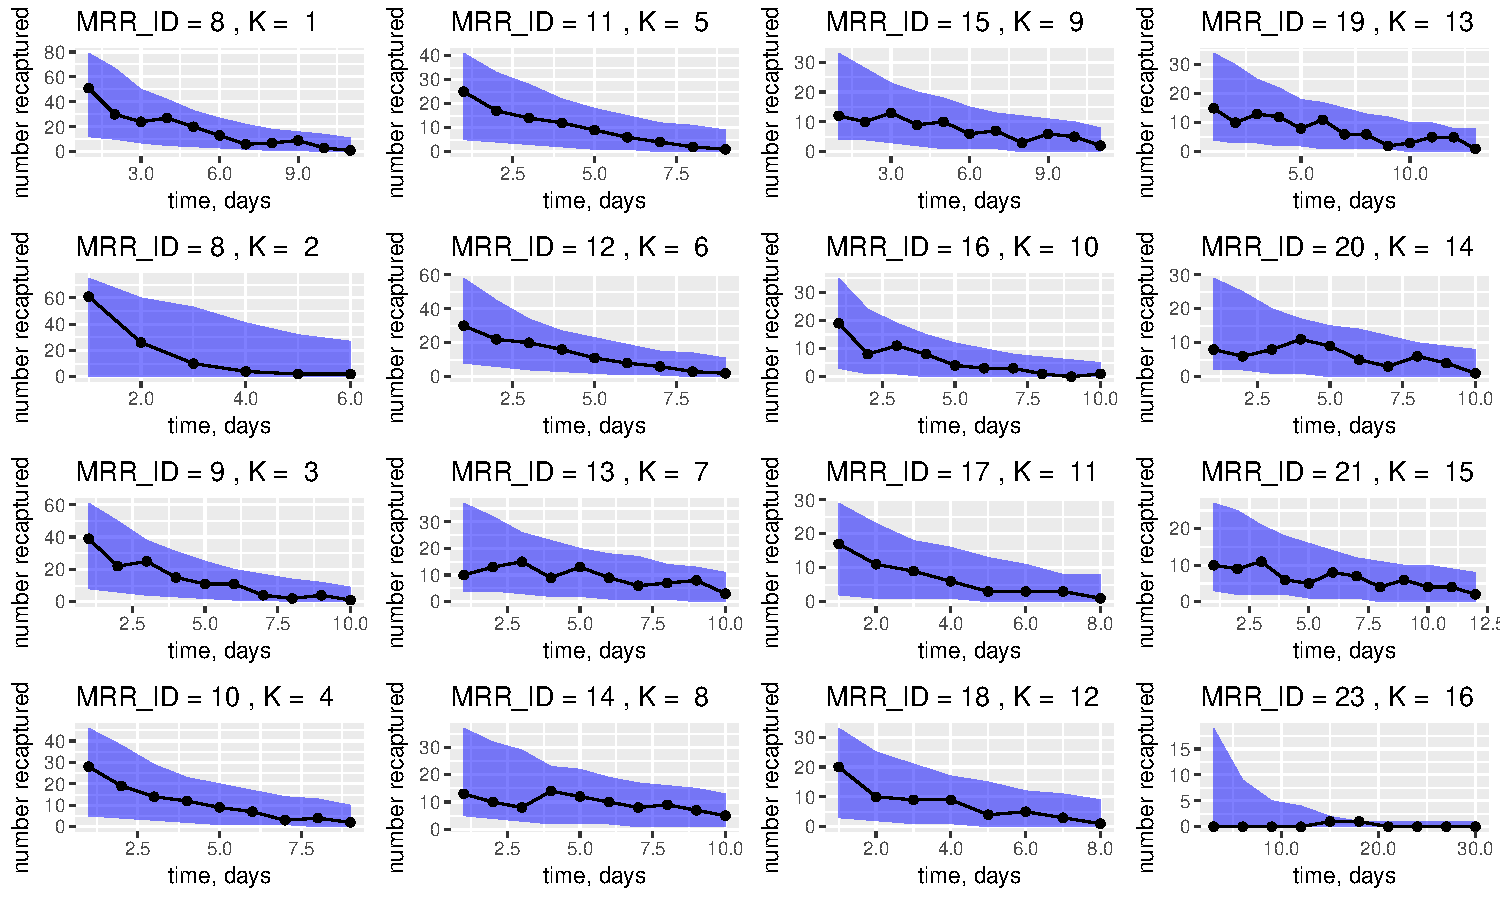
\includegraphics[page=1,scale=.6]{./Figure_files/mrr_ppcs_all}
	\captionof{figure}{The numbers of mosquitoes recaptured (black lines) versus the 95\% central posterior interval of the posterior predictive distribution (blue shading) for a selection of the time series. For the rest of the posterior predictive checks for the MRR models, see the file referenced in the text.}
	\label{fig:mrr_ppc1}
	\par

{%
	\includegraphics[page=2,scale=.6]{./Figure_files/mrr_ppcs_all}
	\captionof{figure}{The numbers of mosquitoes recaptured (black lines) versus the 95\% central posterior interval of the posterior predictive distribution (blue shading) for a selection of the time series. For the rest of the posterior predictive checks for the MRR models, see the file referenced in the text.}
	\label{fig:mrr_ppc2}
	\par
}

{%
	\includegraphics[page=3,scale=.6]{./Figure_files/mrr_ppcs_all}
	\captionof{figure}{The numbers of mosquitoes recaptured (black lines) versus the 95\% central posterior interval of the posterior predictive distribution (blue shading) for a selection of the time series. For the rest of the posterior predictive checks for the MRR models, see the file referenced in the text.}
	\label{fig:mrr_ppc3}
	\par
}




\section{Dissection based estimates}

\subsection{Collection of dissection data}\label{sec:dissection_dissectionData}
A comprehensive search of the literature using Google Scholar (\url{scholar.google.co.uk}) was performed using various combinations of the following keywords: dissection, mosquito, parity, parous, age, and physiological age. No constraints were placed on publication date, location or type. This list was supplemented with a number of author-specific searches for those individuals most prevalent in the literature. In particular we searched for all articles authored by: Charlwood, Muller, Schlein, Samarawickrema, Reisen, Detinova, Polodova, Gillies, and Wilkes. An additional list of potential articles was provided by doing a forward article search on some of the most highly-cited articles in the database: \cite{polovodova1949determination,detinova1962age,gillies1965study,clements1981analysis}. The list of results was then filtered manually by examining the titles and abstracts to produce a candidate list of the articles most likely to contain data on the physiological age of dissected mosquitoes caught in the wild, as determined by the \cite{polovodova1949determination} method.

A relational database was used to store the raw data from the actual experiments, along with the meta-data associated with each of the experiments. In many of the published articles wild mosquitoes were caught and dissected over a period of time, and the raw data thus consists of snapshots of the age structure of the population at regular intervals in time. In the cases where the data was more sparse (fewer than ten individuals, on average, per date), we aggregated across dates and recorded this as a single entry; otherwise we recorded the snapshots of the population at each different date. We record separate series for each species that was captured, or for those that were recorded at separate capture locations (potentially with an alternative collection method), and do not aggregate over these datasets.

For each individual series we recorded the following meta-data: genus, species, collection method, whether or not insecticide was mentioned as being used during or shortly before the time of mosquito collections, and the start and end dates of the experiment. At the article level we recorded the following meta-data: author, year, title, country, location (within country), start and end date, whether insecticide was used during any of the experimental replicates, whether a mrr experiment occurred alongside the dissection study, and the collection location (indoor or outdoor). At either the individual series or article levels we record additional meta-data describing the nature of data collection, for example explaining where the data was contained within the article, whether it was obtained by digitising graphs, and the number of separate dated series. For those few cases ($n=16$ series) where the data was obtained by digitising graphs, we used the WebPlotDigitizer online tool \citep{digitise}.

The data collection method resulted in 568 separate dissection series, across 72 published articles (see Section \ref{sec:appendix_dissectionStudyList} for a list of the studies included in our final dataset). The published datasets cover the period from 1960-2015 with comparable numbers of studies across each decade (Fig. \ref{fig:dissection_timeSeries}). The statistical approach applied to the data relies on the assumption that there is a constant rate of recruitment into the adult population (see Section \ref{sec:dissection_dissectionStats}). If populations fluctuate strongly from month-to-month this assumption will likely be violated. To try to mitigate against such a risk, we aggregate the data across all dates to obtain a single series for each identifier, resulting in 201 such series. To obtain a reasonable level of accuracy on estimates we remove all those individual (aggregated) series where there are fewer than 100 mosquitoes in total in the series. Finally we remove data for any species where there was only one series resulting in 131 series across four genera (\textit{Anopheles}, \textit{Culex}, \textit{Aedes}, and \textit{Mansonia}) and 25 species (Table \ref{tab:dissection_speciesNumbers}). These studies are distributed across a wide range of geographies (Fig. \ref{fig:dissection_map}). The raw data for the dissection analysis are shown in Figures \ref{fig:dissection_exampleData1}, \ref{fig:dissection_exampleData2} and \ref{fig:dissection_exampleData3}.


\begin{figure}[ht]
	\centerline{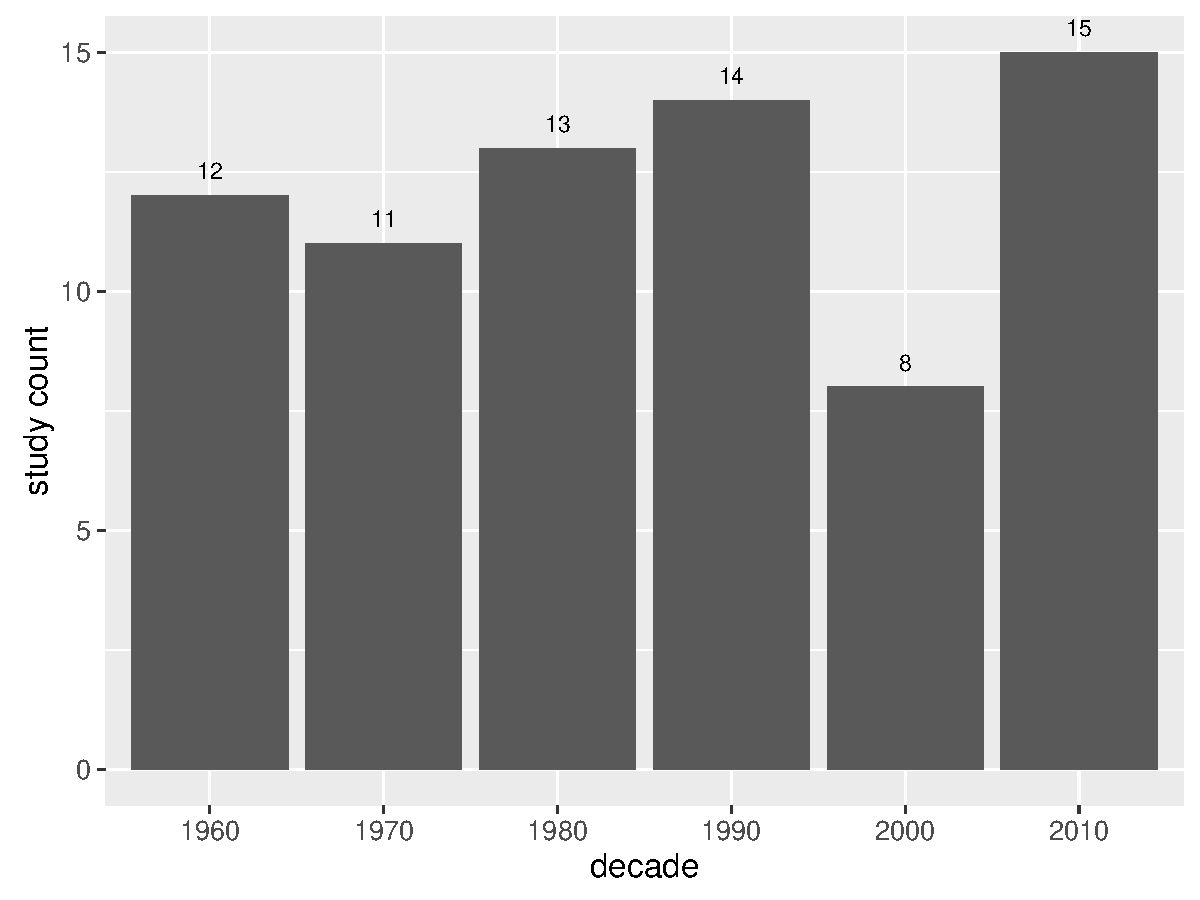
\includegraphics[width=0.8\textwidth]{./Figure_files/dissection_timeSeries.pdf}}
	\caption{\textbf{The numbers of published studies that estimate gonotrophic age by dissection across the study period.}}\label{fig:dissection_timeSeries}
\end{figure}


\begin{figure}[ht]
	\centerline{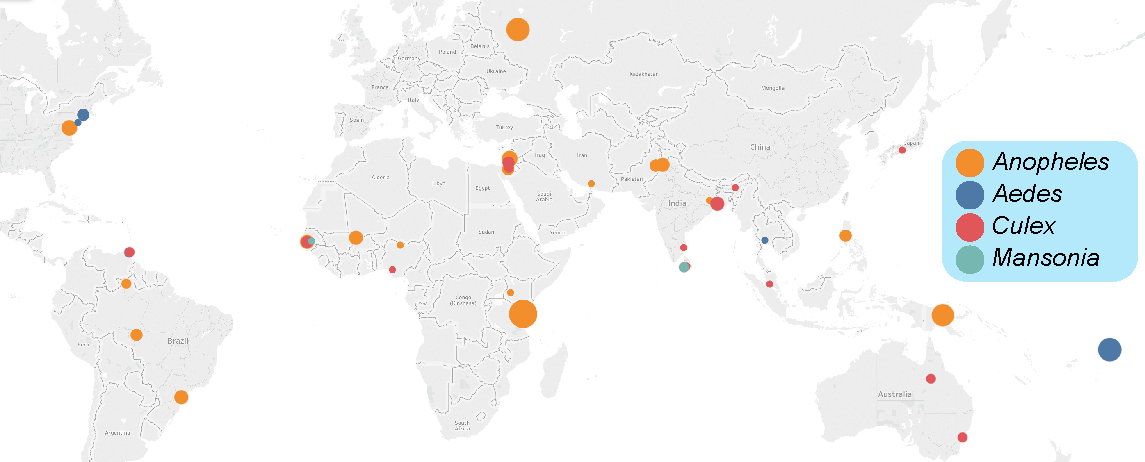
\includegraphics[width=1.25\textwidth]{./Figure_files/dissection_map.pdf}}
	\caption{\textbf{The geographic location of each of the dissection databases included in the meta-analysis.} The area of the bubbles indicates the number of unique data series available.}\label{fig:dissection_map}
\end{figure}

\begin{table}[htbp]
	\centering
	\begin{tabular}{lll}
		\toprule
		\textbf{Genus} & \textbf{Species} & \textbf{Frequency} \\
		\midrule
		\textit{Anopheles} & \textit{gambiae s.l.} & 19 \\
		\textit{Culex} & \textit{quinquefasciatus} & 12 \\
		\textit{Anopheles} & \textit{maculipennis} & 11 \\
		\textit{Anopheles} & \textit{farauti s.l.} & 10 \\
		\textit{Anopheles} & \textit{sergentii} & 8 \\
		\textit{Aedes} & \textit{polynesiensis} & 8 \\
		\textit{Culex} & \textit{pipiens} & 6 \\
		\textit{Anopheles} & \textit{culicifacies} & 5 \\
		\textit{Anopheles} & \textit{darlingi} & 5 \\
		\textit{Anopheles} & \textit{quadrimaculatus} & 5 \\
		\textit{Anopheles} & \textit{stephensi} & 4 \\
		\textit{Anopheles} & \textit{melas} & 4 \\
		\textit{Culex} & \textit{annulirostris} & 4 \\
		\textit{Aedes} & \textit{aegypti} & 3 \\
		\textit{Aedes} & \textit{samoanus} & 3 \\
		\textit{Anopheles} & \textit{minimus} & 3 \\
		\textit{Anopheles} & \textit{rivulorum} & 3 \\
		\textit{Culex} & \textit{thalassius} & 3 \\
		\textit{Mansonia} & \textit{uniformis} & 3 \\
		\textit{Anopheles} & \textit{subpictus} & 2 \\
		\textit{Aedes} & \textit{sollicitans} & 2 \\
		\textit{Aedes} & \textit{vexans} & 2 \\
		\textit{Anopheles} & \textit{bellator} & 2 \\
		\textit{Anopheles} & \textit{cruzii} & 2 \\
		\textit{Culex} & \textit{tritaeniorhynchus} & 2 \\
		\bottomrule
		\textit{\textbf{Anopheles}} &       & \textbf{83} \\
		\textit{\textbf{Culex}} &       & \textbf{27} \\
		\textit{\textbf{Aedes}} &       & \textbf{18} \\
		\textit{\textbf{Mansonia}} &       & \textbf{3} \\
		\bottomrule
		\textbf{Total} &  & \textbf{131} \\
	\end{tabular}%
	\caption{\textbf{The numbers of dissection series for each species or genus included in the overall dataset.}}\label{tab:dissection_speciesNumbers}%
\end{table}%


\begin{table}[htbp]
	\centering
	\footnotesize
	\begin{adjustwidth}{-0.5in}{-0.5in}%
		\begin{tabularx}{1.25\textwidth}{l|ccccc}
			\toprule
			\textbf{Variable} & \textbf{Min} & \textbf{Median} & \textbf{Mean} & \textbf{Max} & \textbf{Standard deviation} \\
			\midrule
			Min age of captures, gonotrophic cycles & 0  & 0  & 0.02  & 1.00  & 0.12 \\
			Median age of captures, gonotrophic cycles & 0  & 1.00  & 0.63  & 2.00  & 0.62 \\
			Mean age of captures, gonotrophic cycles & 0.17  & 0.90  & 1.00  & 3.03  & 0.58 \\
			Max age of captures, gonotrophic cycles & 1.00  & 5.00  & 5.77  & 13.00 & 2.94 \\
			Number captured & 100 & 565 & 1,317 & 14,012 & 1,885 \\
			\bottomrule
		\end{tabularx}%
	\end{adjustwidth}
	\caption{\textbf{Summaries of the characteristics of the 131 individual dissection data series that are included in this analysis.} Note when series are censored (see Section \ref{sec:dissection_censored}) we assume that all mosquitoes dissected over the threshold are of this age when calculating summary statistics.}\label{tab:dissection_summaryStats}
\end{table}

\begin{figure}[ht]
	\centerline{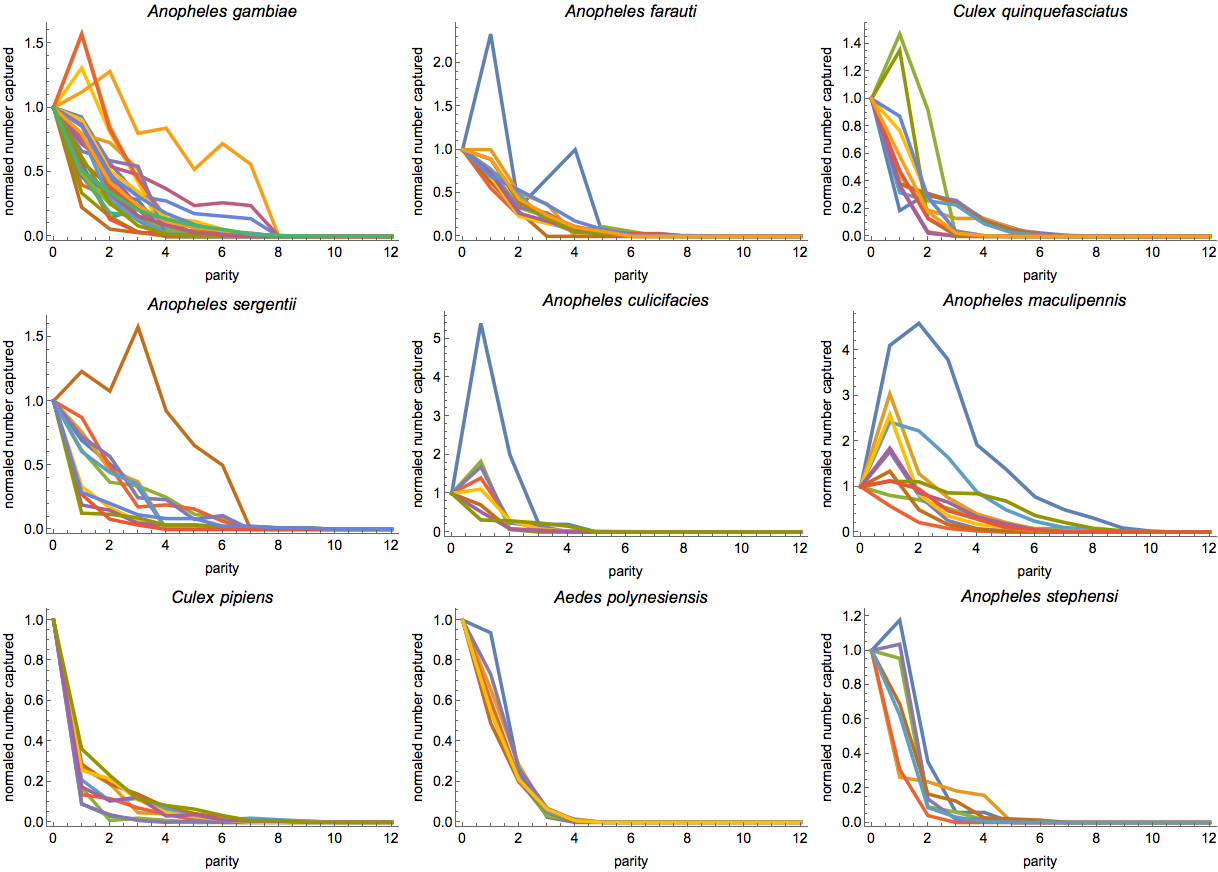
\includegraphics[width=1.3\textwidth]{./Figure_files/dissection_parity_data1.png}}
	\caption{\textbf{The normalised physiological age series for nine species in the database.} Each different coloured line represents an individual series. In each case the count for all ages has been normalised by the nulliparous count. In all cases we do not include any data for censored observations (see Section \ref{sec:dissection_censored}).}\label{fig:dissection_exampleData1}
\end{figure}

\begin{figure}[ht]
	\centerline{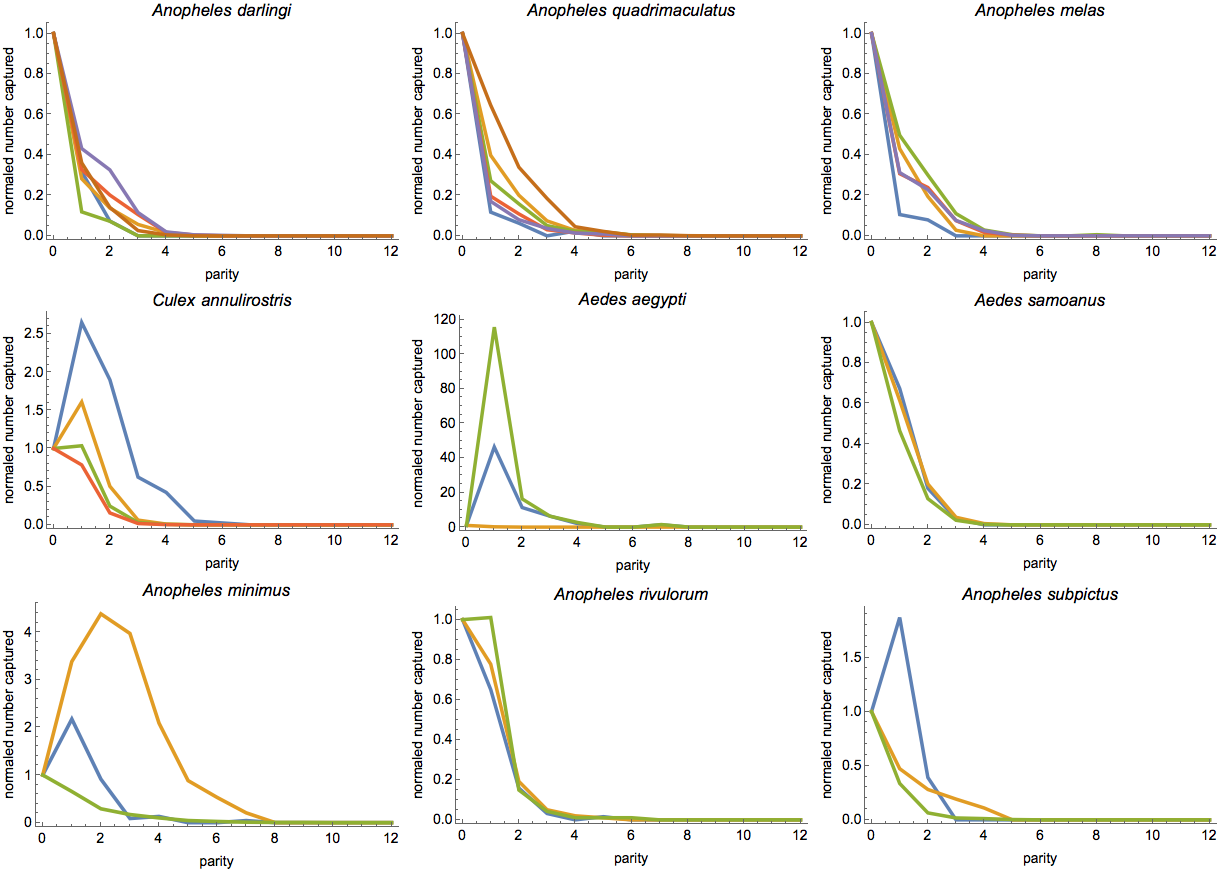
\includegraphics[width=1.3\textwidth]{./Figure_files/dissection_parity_data2.png}}
	\caption{\textbf{The normalised physiological age series for nine species in the database.} Each different coloured line represents an individual series. In each case the count for all ages has been normalised by the nulliparous count. In all cases we do not include any data for censored observations (see Section \ref{sec:dissection_censored}).}\label{fig:dissection_exampleData2}
\end{figure}

\begin{figure}[ht]
	\centerline{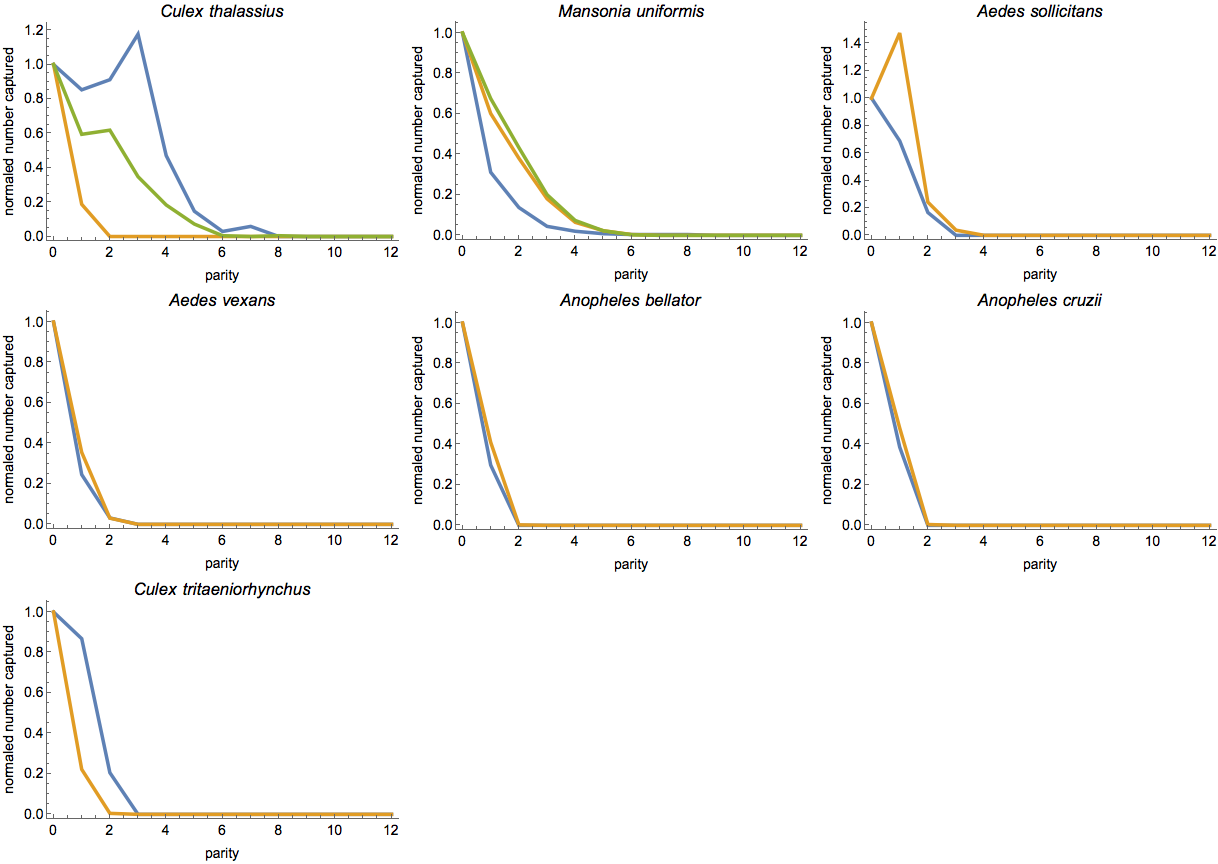
\includegraphics[width=1.3\textwidth]{./Figure_files/dissection_parity_data3.png}}
	\caption{\textbf{The normalised physiological age series for seven species in the database.} Each different coloured line represents an individual series. In each case the count for all ages has been normalised by the nulliparous count. In all cases we do not include any data for censored observations (see Section \ref{sec:dissection_censored}).}\label{fig:dissection_exampleData3}
\end{figure}


\subsection{Statistical analysis of dissection data}\label{sec:dissection_dissectionStats}
We suppose that the number of individuals recruited into the adult female population is constant over time, meaning that the age-structure of the population is stable. Whilst environmental heterogeneity will naturally lead to variation in adult recruitment over time, we hope that by aggregating data across studies undertaken over a range of dates we may reduce the impact of this effect on our results. Suppose that the probability an individual female mosquito survives until age $a$ is given by the survival function $S(a)$, then the number of individuals in the population surviving to this age is given by,
%
\begin{align}\label{eq:dissection_structured}
A(a) = A(0) S(a),
\end{align}
%
where $A(0)$ is the number of female mosquitoes recruited into the population per unit time. Consider one individual experiment where we randomly sample from a wild population that is structured as per eq. (\ref{eq:dissection_structured}). In this case the number of individuals sampled at each age is binomially-distributed,
%
\begin{align}
X(a) \sim \mathcal{B}(A(a),p(a)),
\end{align} 
%
where $p(a)$ is the probability of recapturing a single mosquito of age $a$. In what follows we assume that the probability of capturing a given mosquito is independent of their age, so that $p(a)=p=const$. Since in general $A(a)$ is large and $p(a)$ is small, we can approximate the above using a Poisson distribution,
%
\begin{align}
X(a) \sim \text{Poisson}(A(a)p).
\end{align}
%
However we believe that the assumption of \textit{independent} captures of individual mosquitoes, which underlies the binomial and Poisson models, is likely suspect for the same reasons as for the MRR analysis (see Section \ref{sec:mrr_statistical}). As before we choose to specify a negative binomial sampling distribution that allows for non-independent captures,
%
\begin{align}
X(a) \sim \text{NB}(A(a)p,\kappa),
\end{align} 
%
where we use the parameterisation such that the mean is given by $A(a)p$, and the over-dispersion parameter, $\kappa$, where as $\kappa\rightarrow \infty$ the above sampling distribution approaches a Poisson.

In the field, unfortunately, we do not know the number of mosquitoes recruited into the adult population, $A(a)$, nor the probability of capturing an individual at a given point in time, $p$. Instead we model their product $\Psi=A(0)p$ (the population of adult female mosquitoes of age zero that can be captured) probabilistically resulting in a model,
%
\begin{align}\label{eq:dissertation_negativeBinomial}
X(a) \sim \text{NB}(\Psi S(a),\kappa).
\end{align}
%
The resultant likelihood of a data series consisting of counts: $(y(a_1),y(a_2),...,y(a_R))$, is then calculated by assuming (conditional) independence of the observations,
%
\begin{equation}
\mathcal{L}(y(a_1),y(a_2),...,y(a_R)|S(.),\Psi,\kappa) = \prod\limits_{a=a_1}^{a_R} p(y(a)|S(a),\Psi,\kappa),
\end{equation}
%
where $p(y(a)|S(a),\Psi,\kappa)$ corresponds to the negative binomial probability mass function for a count of $y(a)$ mosquitoes aged $a$ as specified in eqn. (\ref{eq:dissertation_negativeBinomial}), and $R$ is the number of separate physiological age classes in which the count was non-zero.
%
Since we do not know $\Psi$ we must learn it from the data. One approach to estimate this parameter could be use the number of captures of nulliparous mosquitoes, $X(0)$ in place of $\Psi$. We prefer to allow for some uncertainty in this parameter and use the data to estimate its value. However, unfortunately, the negative binomial likelihood allows too much variation in this parameter (because the data are over-dispersed), and instead we specify a likelihood of the form,
%
\begin{align}
X(0) \sim \mathcal{N}(\Psi,\sqrt{\Psi}),
\end{align}
%
solely for the first data point $X(0)$. The above allows for some freedom in $\Psi$ whilst ensuring that the parameter's probability mass lies near enough to $X(0)$ to allow useful model estimates. $\Psi$ is set a uniform prior over the range $[0,\frac{3}{2}X(0)]$.

Since $S(a)$ is monotonically-decreasing we know that, if recruitment to the adult population is constant, then the numbers of nulliparous individuals should exceed the count in subsequent parity states. However in a number of data series there is a relative dearth of nulliparous mosquitoes versus uniparous individuals. This deficiency has been noted in a previously-published study where the authors hypothesise that it is due to the issue of sampling the nulliparous population, since they are more likely to rest outside, compared with parous individuals \citep{gillies1965study}. However there is evidence to suggest that, on average, the first gonotrophic cycle is longer than subsequent cycles (see Section \ref{sec:dissection_gonotrophicData}), meaning that a relative surplus of nulliparous mosquitoes may exist in captured samples \citep{clements1981analysis}.

In our analysis, we chose to remove the counts of nulliparous individuals from the series where the count was low relative to uniparous or higher parity individuals since this may indicate issues with sampling the nulliparous population. Specifically we stipulated that the nulliparous count should exceed 90\% of the count for the uniparous individuals. For those cases where this condition was not met we removed the nulliparous observation and analyse the series of counts for all subsequent pars (uniparous and subsequent parous states).

Here we estimate our model with one of six different survival functions (the same as for the MRR case; Table \ref{tab:mrr_survivalDescription}), each of which makes different assumptions regarding how the force of mortality is affected by mosquito age. To estimate lifespan at the species, genus and overall groupings we then use a hierarchical Bayesian model of the same mathematical form as for the analysis of MRR experiments (see Section \ref{sec:MRR_hierarchical}). However the priors for the analysis of dissection data were modified so that they represented a mean prior lifespan of three gonotrophic cycles, although allowed considerable variation in mean lifespan (Fig. \ref{fig:dissection_lifespanPriorsParity}). The priors used for the over-dispersion parameter ($\kappa$) for the negative binomial likelihood were the same as for the MRR analysis.

To determine whether mosquitoes experience age-dependent mortality we compared the predictive power of each of the models that incorporate a hazard function that depends on age with that from the exponential model. As for the MRR analysis we also used K-Fold cross-validation to perform this comparison, where the data are randomly partitioned into training and test sets (see Section \ref{sec:mrr_kFold}). The model is then fitted to each training set and used to predict the data in the independent test set. Since there are fewer series than for the MRR dataset we used two partitions for each species, where each partition was of roughly the same number of individual series.

\begin{figure}[ht]
	\centerline{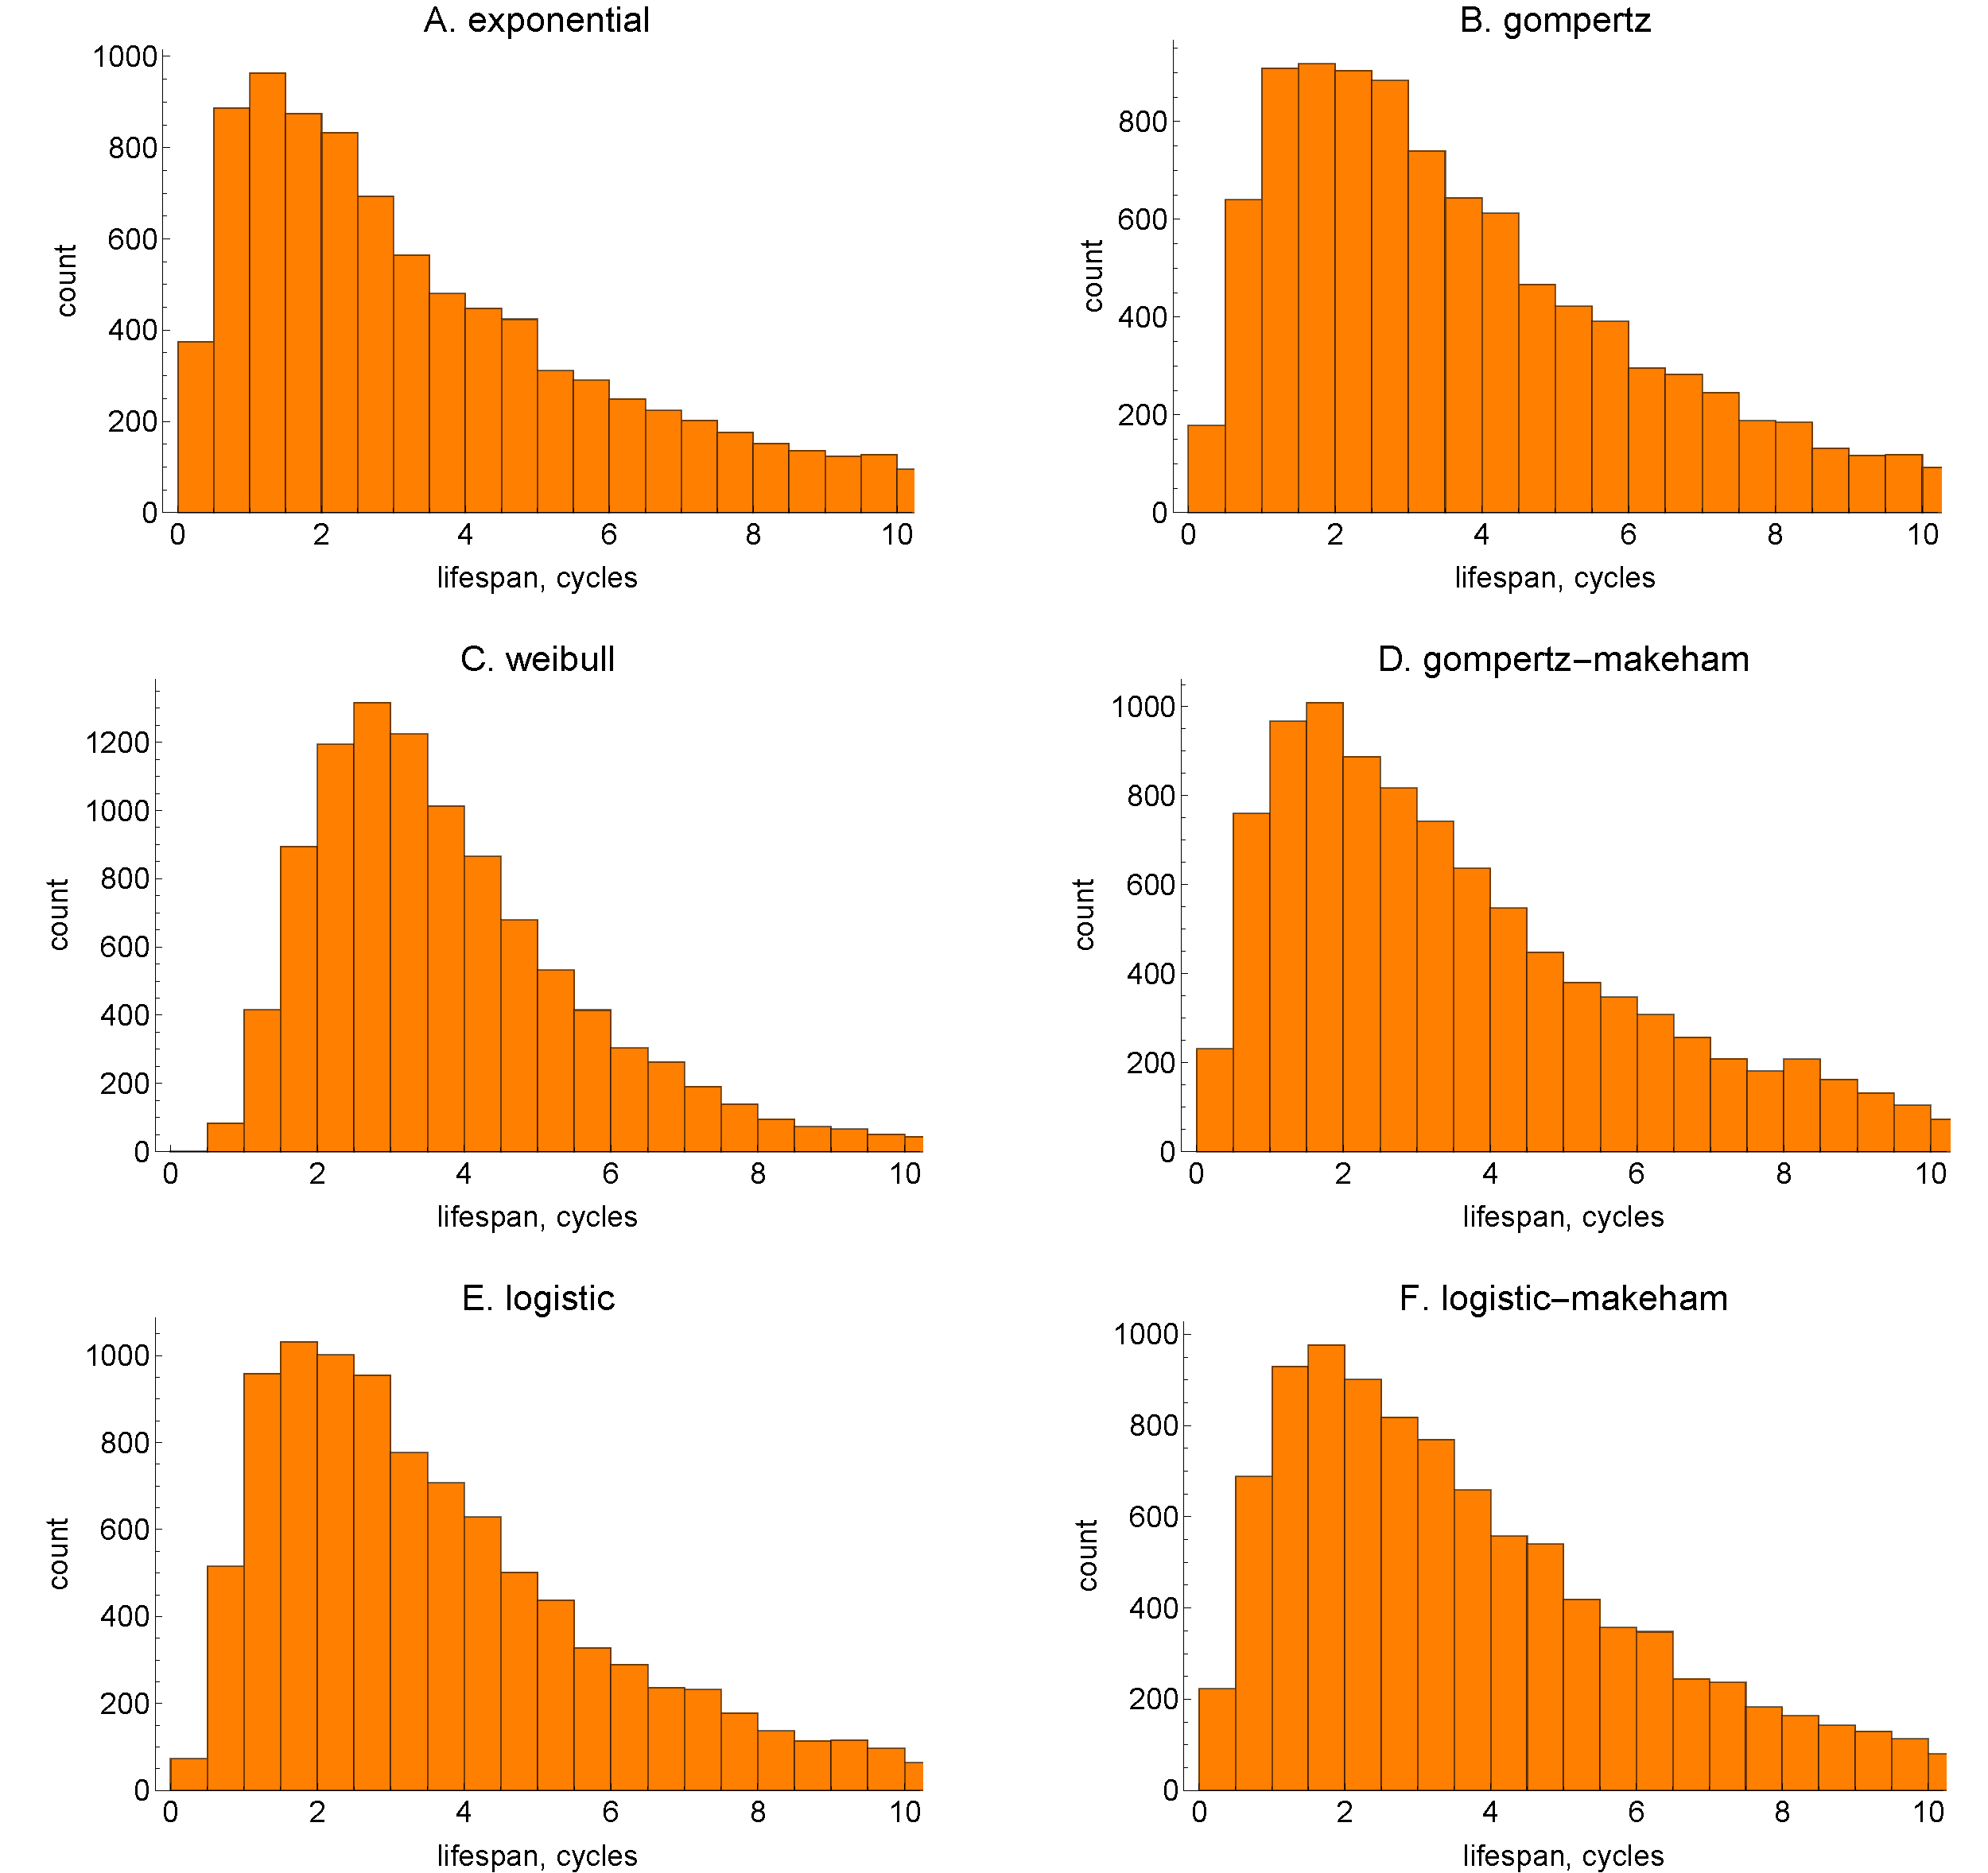
\includegraphics[width=1\textwidth]{./Figure_files/dissection_lifespanPriorsParity.pdf}}
	\caption{\textbf{The priors for mean lifespan used to analyse the data for each of the hierarchical models.} The distributional form of the priors is given in Table \ref{tab:dissection_priors}. In all cases the plots show data for 10,000 samples from the relevant prior distribution.}\label{fig:dissection_lifespanPriorsParity}
\end{figure}

\begin{table}
	\footnotesize
	\noindent\makebox[\textwidth]{%
		\begin{tabularx}{1.2\textwidth}{l|c|X}
			\textbf{Survival function} & \textbf{Physiological age series-level priors} & \textbf{Group-level priors}\\
			\midrule
			Exponential & $\lambda\sim \textnormal{log-normal}(\mu_\lambda,\sigma)$ &$\mu_\lambda \sim N(-1.2,1)\text{,}\; \sigma\sim \textnormal{log-normal}(-2,1)$\\
			\midrule
			Gompertz & $\alpha,\beta\sim$ log-normal$(\mu_{\alpha|\beta},0.2)$ &$\mu_\alpha\sim N(-1.5,1)\text{,}\; \mu_\beta\sim N(-2.5,0.5)$\\
			\midrule
			Weibull & $\alpha,(\beta-1)\sim$  log-normal$(\mu_{\alpha|\beta},0.2)$ &$\mu_\alpha\sim N(-2.5,1)\text{,}\; \mu_\beta\sim N(-4,0.5)$\\
			\midrule
			Gompertz-Makeham & $\alpha,\beta,c\sim$ log-normal$(\mu_{\alpha|\beta|c},0.2)$ &$\mu_\alpha\sim N(-1.4,1)\text{,}\; \mu_\beta\sim N(-3,0.4)\text{,}\; \mu_c\sim N(-4.5,0.5)$\\
			\midrule
			Logistic & $\alpha,\beta,s\sim$  log-normal$(\mu_{\alpha|\beta|s},0.2)$ &$\mu_\alpha\sim N(-1.4,1)\text{,}\; \mu_\beta\sim N(-2,1)\text{,}\; \mu_s\sim N(-3,1)$\\
			\midrule
			Logistic-Makeham & $\alpha,\beta,s,c\sim$ log-normal$(\mu_{\alpha|\beta|s|c},0.2)$ &$\mu_\alpha\sim N(-3,1)\text{,}\; \mu_\beta\sim N(-1.3,1)\text{,}\; \mu_s\sim N(-2,0.5)\text{,}\; \mu_c\sim N(-4,0.5)$\\
			\bottomrule
	\end{tabularx}}\caption{\textbf{The priors used on parameters of each different survival model for the dissection data analysis.} For the exponential model the `group-level' priors were the same for the genus and `overall' models that were also estimated. The exponential model was the only model that was simple enough to allow the scale parameter of the log-normal ($\sigma$) to be estimated by the data. The notation $\alpha,\beta\sim \text{log-normal}(\mu_{\alpha|\beta},0.2)$ means that $\alpha$ and $\beta$ were assigned independent log-normal priors with location parameters $\mu_\alpha$ and $\mu_\beta$ respectively, and a scale parameter of 0.2 in both cases.}\label{tab:dissection_priors}
\end{table}


The estimates of mean mosquito lifespan that we present here (Fig. \ref{fig:dissection_lifetimes_exponential}) resulted from the use of the exponential survival model (i.e. no age dependence). This choice was made because we found limited evidence in support of age-dependent mortality (see `Results'). However, since the priors for each of the survival functions were specified to allow for a wide variety of lifespans (Fig. \ref{fig:dissection_lifespanPriorsParity}) the specific choice of survival function made little difference to resultant estimates (data not shown).

To demonstrate that the results we obtain are not sensitive to the particular form of hierarchical prior structure chosen we also provide estimates of the lifespan for each series analysed separately (i.e. non-hierarchically). To do so we assume priors on the rate parameter of the exponential distribution that provides support over a wide range of possible lifespans (Fig. \ref{fig:dissection_lifespanPrior_individual}A). We also specified a prior on the over-dispersion parameter $\kappa$ that was comparable to the hierarchical case (Fig. \ref{fig:dissection_lifespanPrior_individual}B).


\begin{figure}[ht]
	\centerline{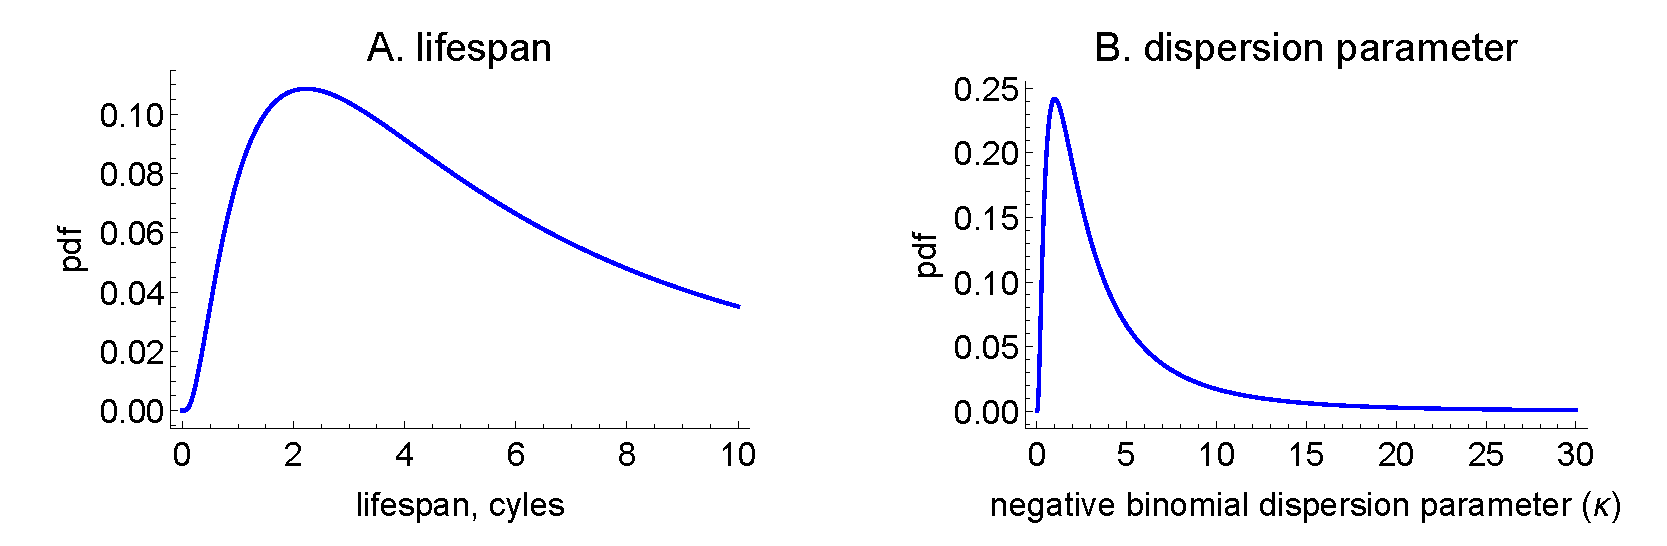
\includegraphics[width=1\textwidth]{./Figure_files/dissection_lifespanPrior_individual.pdf}}
	\caption{\textbf{The priors for A. mean lifespan and B. the over-dispersion parameter used to analyse the individual dissection series.} The prior on the rate parameter of the exponential distribution was $\lambda\sim \text{log-normal}(-1.8,1)$. The prior on the dispersion parameter was $\kappa\sim \text{log-normal}(1,1)$.}\label{fig:dissection_lifespanPrior_individual}
\end{figure}

\subsubsection{Analysis of censored data series}\label{sec:dissection_censored}
Some published studies do not distinguish the number of gonotrophic studies
beyond a threshold, $a_T$ (the more ovariole dilations there are the harder it
is to count them) which is akin to censoring the data. This
censoring involves only a relatively small number of mosquitoes in each
time series (median = 2\%) and so we are confident that these few cases do not substantially affect our inferences. We, however, now describe the statistical model used to describe these instances. In these cases we only know the number, $y(a_T)$, of individuals who were captured and dissected with an estimated physiological age that is greater than or equal to the threshold. Since we do not know the estimated physiological age of individual specimens $i$, we represent this as a parameter, $\aleph_i$, in our statistical model. This means that the joint distribution is a function of $y(a_T)$ different $\aleph_i$ parameters. Since these parameters are not directly of interest, and our chosen MCMC engine, Stan \citep{stan-software:2014}, does not directly allow discrete parameters in models, we marginalise these out of the joint distribution. To do this exactly would require an infinite sum over all the possible ages for all $y(a_T)$ mosquitoes that have been caught whose age exceeds the threshold. Rather than carry out this intractable number of summations we instead make the approximation that all mosquitoes in this group are of the same age $\aleph_i = \aleph,\; \forall i \in (1,...,y(a_T))$. We believe this assumption is justifiable, particularly since the numbers of mosquitoes in each subsequent age category is a strongly-decreasing function of age. This means that whilst we do not know with certainty individuals' ages, it is likely that most will be of the threshold age $a_T$.

This approximation means that to marginalise the parameter $\aleph$ out of the joint distribution, we are only required to do a single summation. Specifically if we have $y(a_T)$ captured individuals of age equal to, or exceeding, some threshold age, $a_T$, the probability of these observations is given by,
%
\begin{align}
q(y(a_T)|S(.),\Psi,\kappa) &= \sum_{\aleph=a_T}^{\infty} p(y(a_T),\aleph|S(\aleph),\Psi,\kappa)\\
&= \sum_{\aleph=a_T}^{\infty} p(y(a_T)|S(\aleph),\Psi,\kappa) \times p(\aleph)
\end{align}
%
where $q(y(a_T)|S(\aleph),\Psi,\kappa)$ is the probability of observing $y(a_T)$ counts for mosquitoes of an age $\aleph$. In practice, since we do not believe mosquitoes live for longer than 20 gonotrophic cycles (the maximum observed in the data was 13), we cut-off the summation at this point, and assume that the discrete prior probability distribution $p(\aleph)$ is uniform over this range. The overall likelihood for the cases where the series are censored therefore has the form,
%
\begin{equation}
\mathcal{L}(y(a_1),y(a_2),...,y(a_T-1),y(a_T)|S(.),\Psi,\kappa) = \left(\prod\limits_{a=a_1}^{a_T-1} p(y(a)|S(a),\Psi,\kappa)\right) q(y(a_T)|S(\aleph),\Psi,\kappa).
\end{equation}
%
In practice, the number of mosquitoes captured in those series that are censored represents a small percentage of total captures (the median is approximately 2\%), and so the effect of the $q(.)$ term above is likely minimal on resultant inferences.

\subsection{Model estimation by MCMC}\label{sec:dissection_MCMC}
As for the MRR analysis, we used \textit{Stan} software \citep{carpenter2016stan} to sample from the posterior distributions of model parameters.

To judge convergence of the sampling algorithm to the posterior density, we calculated $\hat{R}$ across all Markov chains -- a ratio that compares the between-chain variation to that within each chain that is commonly used to measure convergence in MCMC \citep{gelman1992inference}. For each model, we ran 16 independent Markov chains with 200 iterations per chain, discarding the first half of these iterations as warm-up \citep{gelman2014bayesian}. After running the algorithm for the given number of observations, $\hat{R}<1.1$ for all model parameters. We also ensured that across each MCMC run the number of divergent iterations (that can bias the MCMC away from the true posterior density) was minimal. In the majority of cases, the number of divergent iterations was far fewer than 1\% of the total number of samples.

The model used to estimate the lifespan in terms of gonotrophic cycles is provided below.

\begin{minted}{stan}
data{
int N; // number of obs
int K; // number of time series
int Y[N]; // number captured
int S[K]; // length of each series
int threshold[K]; // age of censoring; if -1 then no censoring
int Pos[K]; // position of start of each series in Y
int species[K]; // index variable of species
int nSpecies; // number of species
}

parameters{
real<lower=0> PopSize[K];
real<lower=0> alpha[K];
real alpha_mean[nSpecies];
real<lower=0> alpha_sigma[nSpecies];
real<lower=0> kappa[K];
real<lower=0> p[nSpecies];
}

model{
// Likelihood
for(i in 1:K){
  for(t in 2:S[i]){
    // uncensored
    if(threshold[i] < 0)
      Y[Pos[i]+t-1] ~ neg_binomial_2(PopSize[i] *
			exp(-alpha[i] * (t-1)), kappa[i]);
    // censoring
    else{
      if((t-1) < threshold[i])
        Y[Pos[i]+t-1] ~ neg_binomial_2(PopSize[i] *
			exp(-alpha[i] * (t-1)), kappa[i]);
      else{
        real lLogProb[20];
        for(j in 1:20){
          lLogProb[j] = neg_binomial_2_lpmf(Y[Pos[i]+t-1] |
			PopSize[i] * exp(-alpha[i] * (t-1)),
			kappa[i]);
        }
        target += log_sum_exp(lLogProb);
      }
    }
  }  
}

// Priors
for(i in 1:K){
  int aSpecies;
  aSpecies = species[i];
  Y[Pos[i]] ~ normal(PopSize[i], sqrt(PopSize[i]));
  alpha[i] ~ lognormal(alpha_mean[aSpecies],
  			alpha_sigma[aSpecies]);
  kappa[i] ~ exponential(p[aSpecies]);
}

alpha_mean ~ normal(-1.2, 1);
alpha_sigma ~ lognormal(-2, 1);
p ~ lognormal(1, 1);
}

generated quantities{
real alpha_average[nSpecies];
for(i in 1:nSpecies)
  alpha_average[i] = lognormal_rng(alpha_mean[i],alpha_sigma[i]);
}
\end{minted}

\subsection{Model checking}
As for the MRR experiments, we simulated from the posterior predictive distribution for each series of dissection data. In the majority of the cases, the capture data lay within the 95\% posterior predictive intervals, indicating that our model was a good fit to the data (see Figures \ref{fig:dissection_ppc_all1}, \ref{fig:dissection_ppc_all2} \&  \ref{fig:dissection_ppc_all3} and the attached file, \verb|dissection_ppcs_all.pdf| for the full graphs).

\newgeometry{scale=0.8}
\thispagestyle{empty}
{%
	\centering
	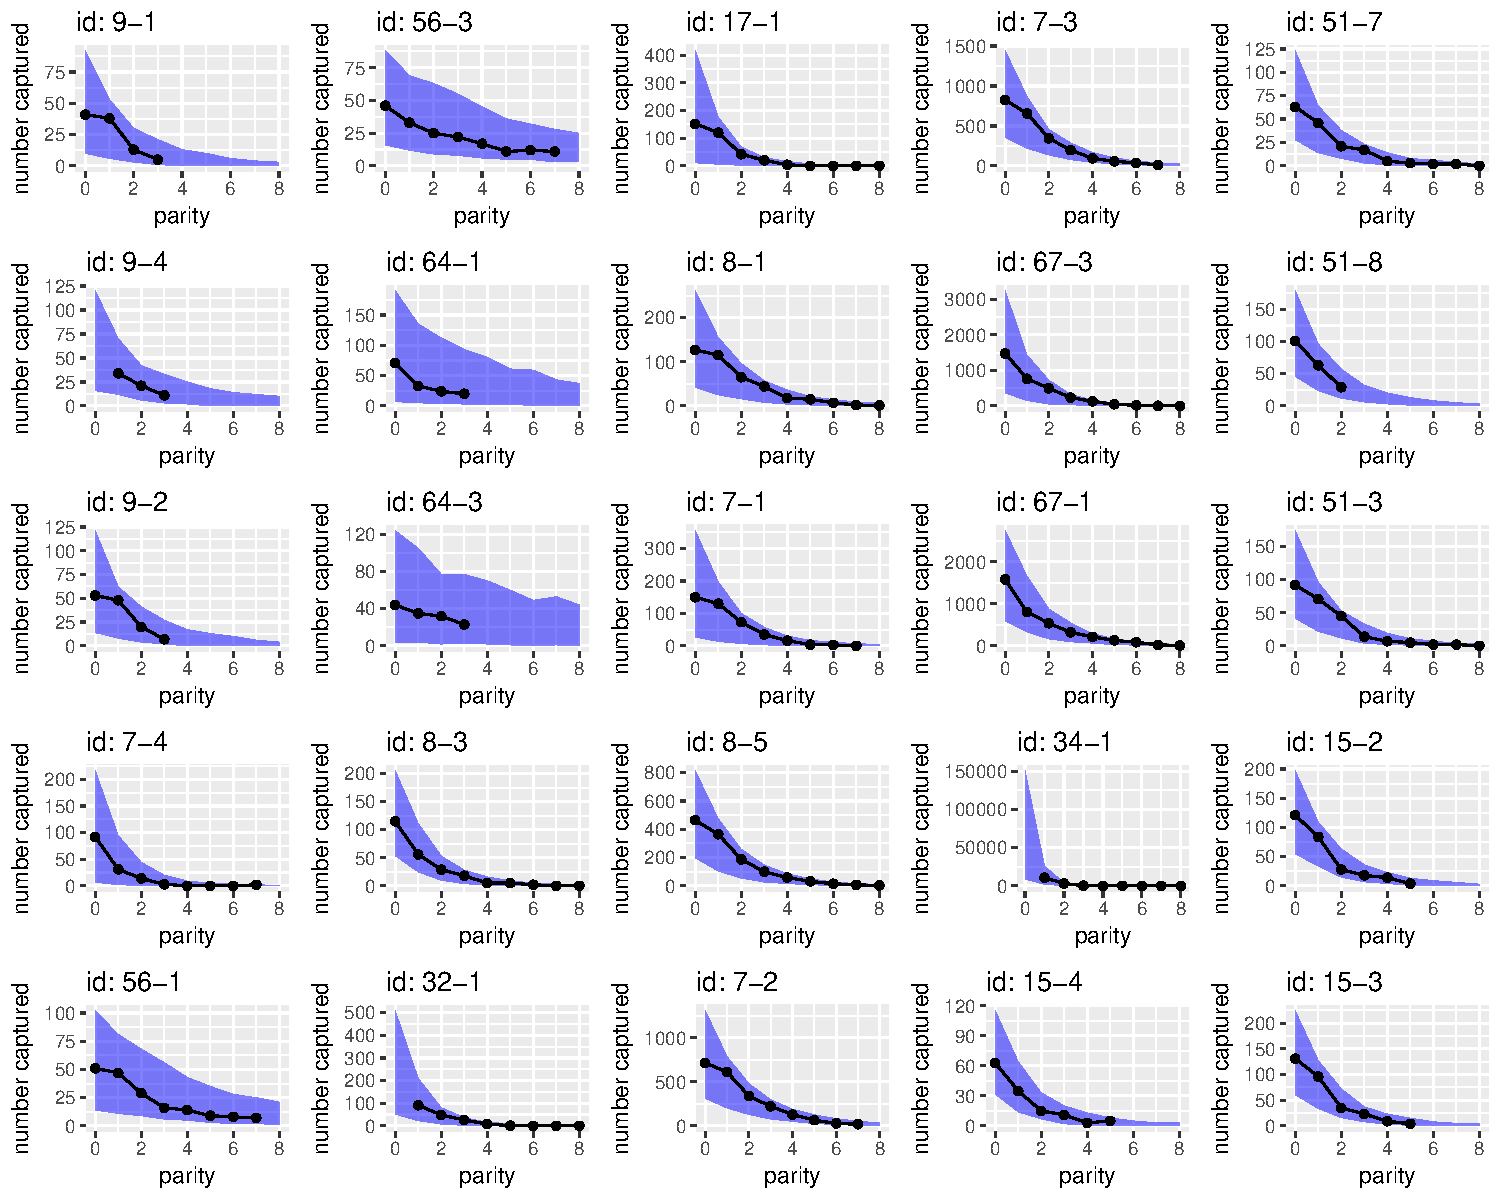
\includegraphics[page=1,scale=.7]{./Figure_files/dissection_ppcs_all}
	\captionof{figure}{\textbf{The numbers of mosquitoes recaptured (black lines) versus the 95\% central posterior interval of the posterior predictive distribution (blue shading) for a selection of the dissection series.} The titles correspond to the unique combination of "identifier - physiological-experiment-id" in the database. For the rest of the posterior predictive checks for the dissection data models, see the file referenced in the text.}
	\label{fig:dissection_ppc_all1}
	\par
}
\restoregeometry

\newgeometry{scale=0.8}
\thispagestyle{empty}
{%
	\centering
	\includegraphics[page=2,scale=.7]{./Figure_files/dissection_ppcs_all}
	\captionof{figure}{\textbf{The numbers of mosquitoes recaptured (black lines) versus the 95\% central posterior interval of the posterior predictive distribution (blue shading) for a selection of the dissection series.} The titles correspond to the unique combination of "identifier - physiological-experiment-id" in the database. For the rest of the posterior predictive checks for the dissection data models, see the file referenced in the text.}
	\label{fig:dissection_ppc_all2}
	\par
}
\restoregeometry

\newgeometry{scale=0.8}
\thispagestyle{empty}
{%
	\centering
	\includegraphics[page=3,scale=.7]{./Figure_files/dissection_ppcs_all}
	\captionof{figure}{\textbf{The numbers of mosquitoes recaptured (black lines) versus the 95\% central posterior interval of the posterior predictive distribution (blue shading) for a selection of the dissection series.} The titles correspond to the unique combination of "identifier - physiological-experiment-id" in the database. For the rest of the posterior predictive checks for the dissection data models, see the file referenced in the text.}
	\label{fig:dissection_ppc_all3}
	\par
}
\restoregeometry


\subsection{Data collection of gonotrophic cycle duration}\label{sec:dissection_gonotrophicData}
To convert the estimates of lifespan in physiological age into chronological age we require estimates of the duration of the gonotrophic cycle. To determine this characteristic we conducted a meta-analysis of previously-published studies that estimate the duration of the gonotrophic cycle. A search of the literature using Google Scholar (\url{scholar.google.co.uk}) was performed using the search term: `gonotrophic cycle duration'. The list of articles was then supplemented with a list of references discussed by \cite{silver2007mosquito}. Based on the abstracts of the resultant list of published studies we then decided whether to search each article for estimates of the duration of the gonotrophic cycle. Overall 79 separate estimates of this parameter were found across 42 published articles (see Section \ref{sec:appendix_gonotrophicDurationStudyList} for a list of the studies included in our dataset). Along with information about the estimates we also recorded study and series meta-data, including the location of the study, the method used for estimation, the species and genus, as well as the temperatures and/or seasons in which the experiments were carried out. The methods used to estimate gonotrophic cycle duration in the literature largely fell into two distinct categories: those based on MRR studies ($n=29$); and those based on observations of mosquitoes in a laboratory setting ($n=42$). In the MRR studies estimates are made of the duration of gonotrophic cycles by dissecting recaptured mosquitoes at each time point using the method of \cite{polovodova1949determination} to count ovariolar dilations. For the laboratory studies the duration of gonotrophic cycles is determined more directly by observing the time taken for mosquitoes to mate then blood-feed and finally oviposit.

Along with point estimates of the parameter we also collected information about the uncertainty in the estimates (if available). In many articles the duration of the gonotrophic cycle was estimated separately for the first versus subsequent cycles, and these estimates were recorded separately. Raw estimates of gonotrophic cycle duration were obtained for species across four different genera (\textit{Aedes}, \textit{Anopheles}, \textit{Culex} and \textit{Masonia}), although there was a bias towards \textit{Anopheles} with $n=47$ estimates out of the total of 79 (Fig. \ref{S-fig:dissection_gonotrophicCycleRaw}). 

Since we collected data on the method used to estimate the duration of the gonotrophic cycle we show the raw estimates for the two most common approaches: MRR and laboratory (Fig. \ref{S-fig:dissection_gonotrophicCycleRaw_MRRVsLab}). From these results it is evident that the estimates from the laboratory studies are, on average, higher than those using the MRR method.

\subsection{Statistical analysis of gonotrophic cycle data}\label{sec:dissection_gonotrophicMethod}
As discussed in Section \ref{sec:dissection_gonotrophicData}, there was considerable study-level heterogeneity in the information provided for the estimates of the gonotrophic cycle duration. A number of studies ($n=24$) provided no estimates of uncertainty in gonotrophic cycle duration, whereas the rest gave some indication of confidence or alternatively a range of possible estimates. However the types of uncertainty intervals that were specified varied considerably from study to study, from the vague (but common)  `4-6 days' to the more helpful `5$\pm 1$ day (95\% confidence interval)'. 

The heterogeneous nature of the gonotrophic cycle estimates requires a method that explicitly accounts for this characteristic of the data. We decided to model the estimates as representing quantiles from an underlying normal distribution that represents uncertainty over possible durations of the gonotrophic cycle. In those circumstances where lower, central and upper bounds were given explicitly the data was fairly symmetric and so we believe assuming the observations come from an unskewed normal distribution is reasonable. Explicitly we treated each type of uncertainty interval as follows,

\begin{itemize}
	\item Simple range, for example, `4-6 days': treat the lower and upper bounds as the 2.5\% and 97.5\% quantiles of a normal distribution.
	\item Confidence intervals, `5$\pm 1$ day (95\% confidence interval)': treat the lower and upper bounds as the relevant quantiles of a normal distribution.
	\item Point estimates, for example `5 days': treat this as the median of a normal distribution.
\end{itemize}

The benefit of this approach is that we can convert the quantiles from our normal distribution parameterised by a mean ($\mu$) and standard deviation ($\sigma$) to equivalent quantiles from a standard normal,
%
\begin{align}
Z_{50} = \frac{G_{50} - \mu}{\sigma},
\end{align}
%
where $Z_{50}$ and $G_{50}$ indicate 50\% quantiles from a standard normal distribution and a normal distribution respectively. By manipulating the above expression we obtain the following,
%
\begin{align}
G_{50} = \sigma Z_{50} + \mu,
\end{align}
%
which forms a straight line in $(Z,G)$ space with slope $\sigma$ and y-intercept $\mu$. Therefore by plotting the raw observations of $(Z,G)$ quantiles then estimating a linear regression line we can characterise the underlying $\mathcal{N}(\mu,\sigma)$ distribution from which we assume they are drawn.

Due to the relative unavailability of estimates for gonotrophic cycle duration across the different genera we generated a single distribution to represent the uncertainty in this parameter by pooling all the data. This was justified because there was not found to be significant variation in the 1st gonotrophic cycle duration (ANOVA: $F_{3,75}=2.6,p>0.05$).

Using the collected data, we estimated that the first gonotrophic cycle duration was $\mathcal{N}(4.26, 0.38)$ and, for subsequent cycles, $\mathcal{N}(3.85, 0.35)$.

\subsection{Conversion of lifespan from physiological to calendar age}\label{sec:dissection_conversion}
The estimates of lifespan produced from analysing the dissection data are in terms of physiological age (the number of gonotrophic cycles undertaken). To allow comparison with the estimates from the MRR studies (Fig. \ref{fig:mrr_lifespans}) as well as produce more useful estimates to inform disease transmission dynamical models we convert these estimates to calendar days. To do this we use the estimated parameters of the normal densities that we have assumed represent uncertainty in gonotrophic cycle duration (see Section \ref{sec:dissection_gonotrophicMethod}) and use them to convert our posterior samples of mean physiological lifespan $(L^p_1,...,L^p_S)$ to lifespan in calendar ages $(L^c_1,...,L^c_S)$. To do this we iterate the following for all $i\in (1,...,S)$ posterior samples,

\begin{enumerate}
	\item Sample $G_{1i} \sim \mathcal{N}(\mu_{1i},\sigma_{1i})$, to obtain a duration for the 1st gonotrophic cycle.
	\item Sample $G_{2i} \sim \mathcal{N}(\mu_{2i},\sigma_{2i})$, to obtain a duration for subsequent gonotrophic cycles.
	\item If $L^p_i > 1$, the mean lifespan is longer than one gonotrophic cycle:
	\subitem then $L^c_i = G_{1i} + G_{2i} \times (L^p_i - 1)$.
	\item Else:
	\subitem then $L^c_i = G_{1i}\times L^p_i$.
\end{enumerate}

In the using the above methodology to convert from physiological to calendar age we implicitly assume that for each gonotrophic cycle after the first that the cycles are of the same length (we choose one $G_{2i}$ per sample). However since we allow a different $G_{2i}$ for each sample we nonetheless believe that the above approach allows for sufficient uncertainty in the estimates of subsequent gonotrophic cycle durations. If instead we believed that significant variation in gonotrophic cycle occurred within a particular mosquito's life (as well as between mosquitoes) then we could draw a new value of $G_{2i}$ for each subsequent cycle. This produces results with a little more uncertainty than previously (data not shown).

\section{Detinova parity analysis}\label{sec:detinova}
\cite{detinova1962age} provided an alternative approach to estimate the lifespan of individual specimens, based on sampling the parous rate in a population (the proportion of adult females that have laid eggs) using dissection to determine parity of each specimen. In what follows, we follow the derivation given by \cite{davidson1954estimation}, to determine an expression for the proportion of nulliparous mosquitoes in terms of the gonotrophic cycle length $G$, here assumed the same for each cycle subsequent to an adult emerging. If a constant daily survival rate $p$ is assumed, the proportion of emerging adults surviving to become parous is $p^G$. If the rate of recruitment into the adult classes is constant over time, the proportion of nulliparous mosquitoes is,
%
\begin{equation}\label{eq:detinova}
\begin{aligned}
\mathbb{n} &= \frac{p^G}{p^G + p^{2G} + p^{3G} + \cdots}\\
&= p^G / \frac{p^G}{1-p^G}\\
&= 1-p^G.
\end{aligned}
\end{equation}
%
The daily survival rate can hence be calculated by inverting eq. (\ref{eq:detinova}): $p = \sqrt[G]{\mathcal{P}}$, where $\mathcal{P}=1-\mathbb{n}$ is the proportion parous sampled from the population.

\cite{massey2016global} provide a global database of bionomic quantities for the dominant vector species of malaria. This database contains the number of parous and nulliparous samples in studies where Detinova's dissection approach was applied to field caught speciments ($n=1490$ non-missing observations for total number of parous individuals) across Africa ($n=778$), Asia ($n=549$) and the Americas ($n=163$). 

We estimated lifespan at the species and complex / subgroup level (hereafter denoted as \textit{s.l.}) using a Bayesian hierarchical framework. We denote this grouping variable by $s$ in what follows. The number of parous individuals $X_i^{\{s\}}$ in sample $i$ (consisting of individuals belonging to group $s$) was modelled by a binomial sampling distribution,
%
\begin{equation}
X_i^{\{s\}} \sim \mathcal{B}(N, \mathcal{P}_i^{\{s\}}),
\end{equation}
%
where $N$ is the sample size and $\mathcal{P}_i^{\{s\}}$ is the proportion parous in sample $i$ for group $s$. A hierarchical prior structure was used for the parous proportion in each sample,
%
\begin{equation}
\mathcal{P}_i^{\{s\}}\sim \text{beta}\left(\phi^{\{s\}} \kappa^{\{s\}}, (1-\phi^{\{s\}})\kappa^{\{s\}}\right),
\end{equation}
%
where $0\leq\phi^{\{s\}}\leq 1$ is the mean parous proportion and $\kappa^{\{s\}}>1$ is a concentration parameter (both of which are group-specific).

The priors we used in this model were: $\phi\sim \text{beta}(20, 14)$ and $\kappa\sim \text{Pareto}(1, 1.5)$. These were chosen because this yielded a prior predictive distribution with a median value close to 10 (see Fig. \ref{fig:detinova_priors}).

\begin{figure}[ht]
	\centerline{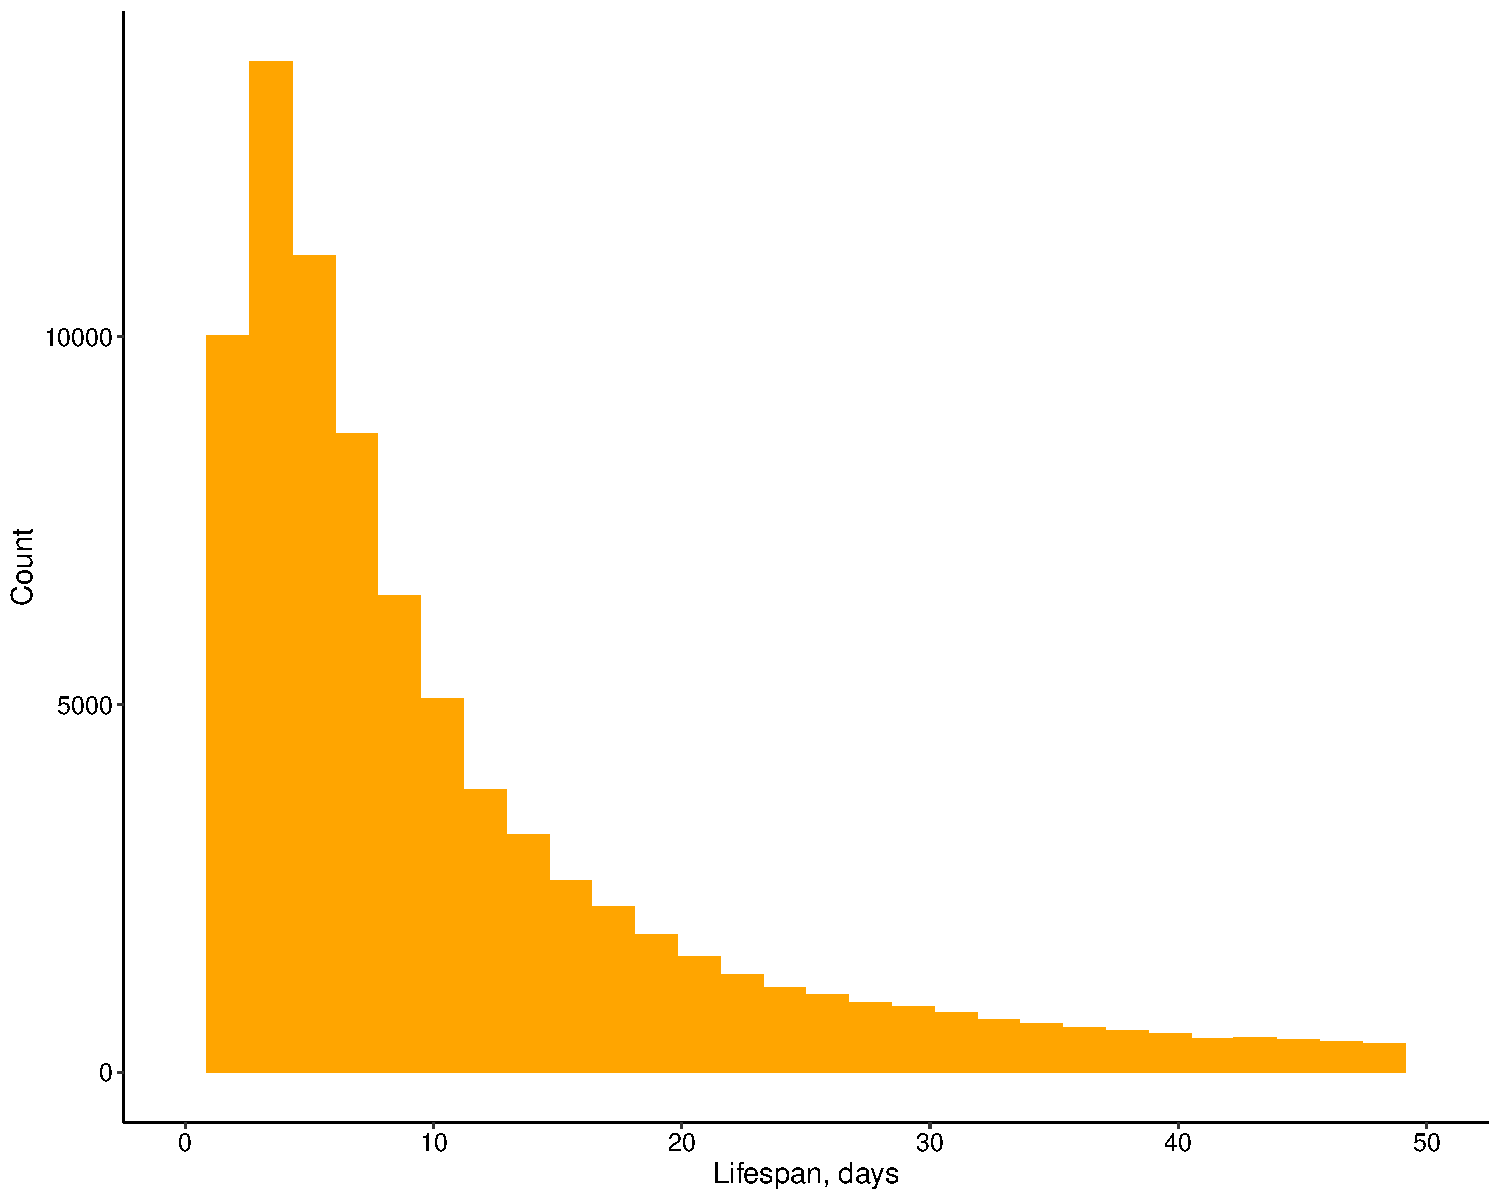
\includegraphics[width=1\textwidth]{./Figure_files/detinova_prior_predictive.pdf}}
	\caption{\textbf{The prior predictive distribution of lifespan for the analysis of Detinova parity data.} Here, we used the estimates of first gonotrophic cycle duration, $G\sim \mathcal{N}(4.26, 0.38)$, resultant from the approach outlined in section \ref{sec:dissection_gonotrophicMethod}, to convert physiological survival to calendar days. The figure shows 100,000 samples from the prior predictive distribution.}\label{fig:detinova_priors}
\end{figure}

The Stan code used to fit the hierarchical model to data is shown below.

\begin{minted}{stan}
data{
  int N;
  int X[N];
  int num[N];
  int species[N];
  int K;
}

parameters{
  vector<lower=0, upper=1>[N] theta;
  vector<lower=0, upper=1>[K] phi;
  vector<lower=1>[K] kappa;
}

model{
  for(i in 1:N){
    X[i] ~ binomial(num[i], theta[i]);
    theta[i] ~ beta(phi[species[i]] * kappa[species[i]],
                    (1 - phi[species[i]]) * kappa[species[i]]);
  }
  kappa ~ pareto(1, 1.5);
  phi ~ beta(20, 14);
}
\end{minted}


\subsection{Model checking}
To check the fit of the models to data, we simulated from the posterior predictive distribution for each grouping used in analysis. This means that we have two sets of posterior predictive figures: those where the check was performed at the species level; and those corresponding to the complex or subgroup level. In each of these figures, we plot observed parity versus quantiles of posterior predicted parity (black vertical error bars). The following describes which figures correspond to which geography and species grouping.

\begin{itemize}
	\item \textbf{Africa}: the complex-level posterior predictive distribution graph is shown in Figure \ref{fig:detinova_ppcs_africa_grouped}; the species-level graph in Figure \ref{fig:detinova_ppcs_africa_species}.
	\item \textbf{Americas}: the complex-level posterior predictive distribution graph is shown in Figure \ref{fig:detinova_ppcs_americas_grouped}; the species-level graph in Figure \ref{fig:detinova_ppcs_americas_species}.
	\item \textbf{Asia}: the complex-level posterior predictive distribution graph is shown in Figure \ref{fig:detinova_ppcs_asia_grouped}; the species-level graph in Figure \ref{fig:detinova_ppcs_asia_species}.
\end{itemize}

In most cases, the posterior predictive distribution overlaps with the observed data (when the black error bars overlap with the orange ${\text{observed}=\text{predicted}}$ lines), indicating that the model was a reasonable fit to the data. For the most extreme observations of parity - when either very few or most samples where parous - however, the model-estimated parity was moved closer to the grand mean. This effect is illustrated in the figures by the linear regression line fitted to the data (blue lines). In almost all cases, the regression line had a lower gradient than the orange ${\text{observed}=\text{predicted}}$ lines, indicating a degree of ``shrinkage to the mean''. This shrinkage to the mean is a common and desirable product of using hierarchical models and can improve the robustness of results by reducing the influence of outliers \citep{lambert2018student}. As such, we do not view this as evidence of model misfit.

\begin{figure}[ht]
	\centerline{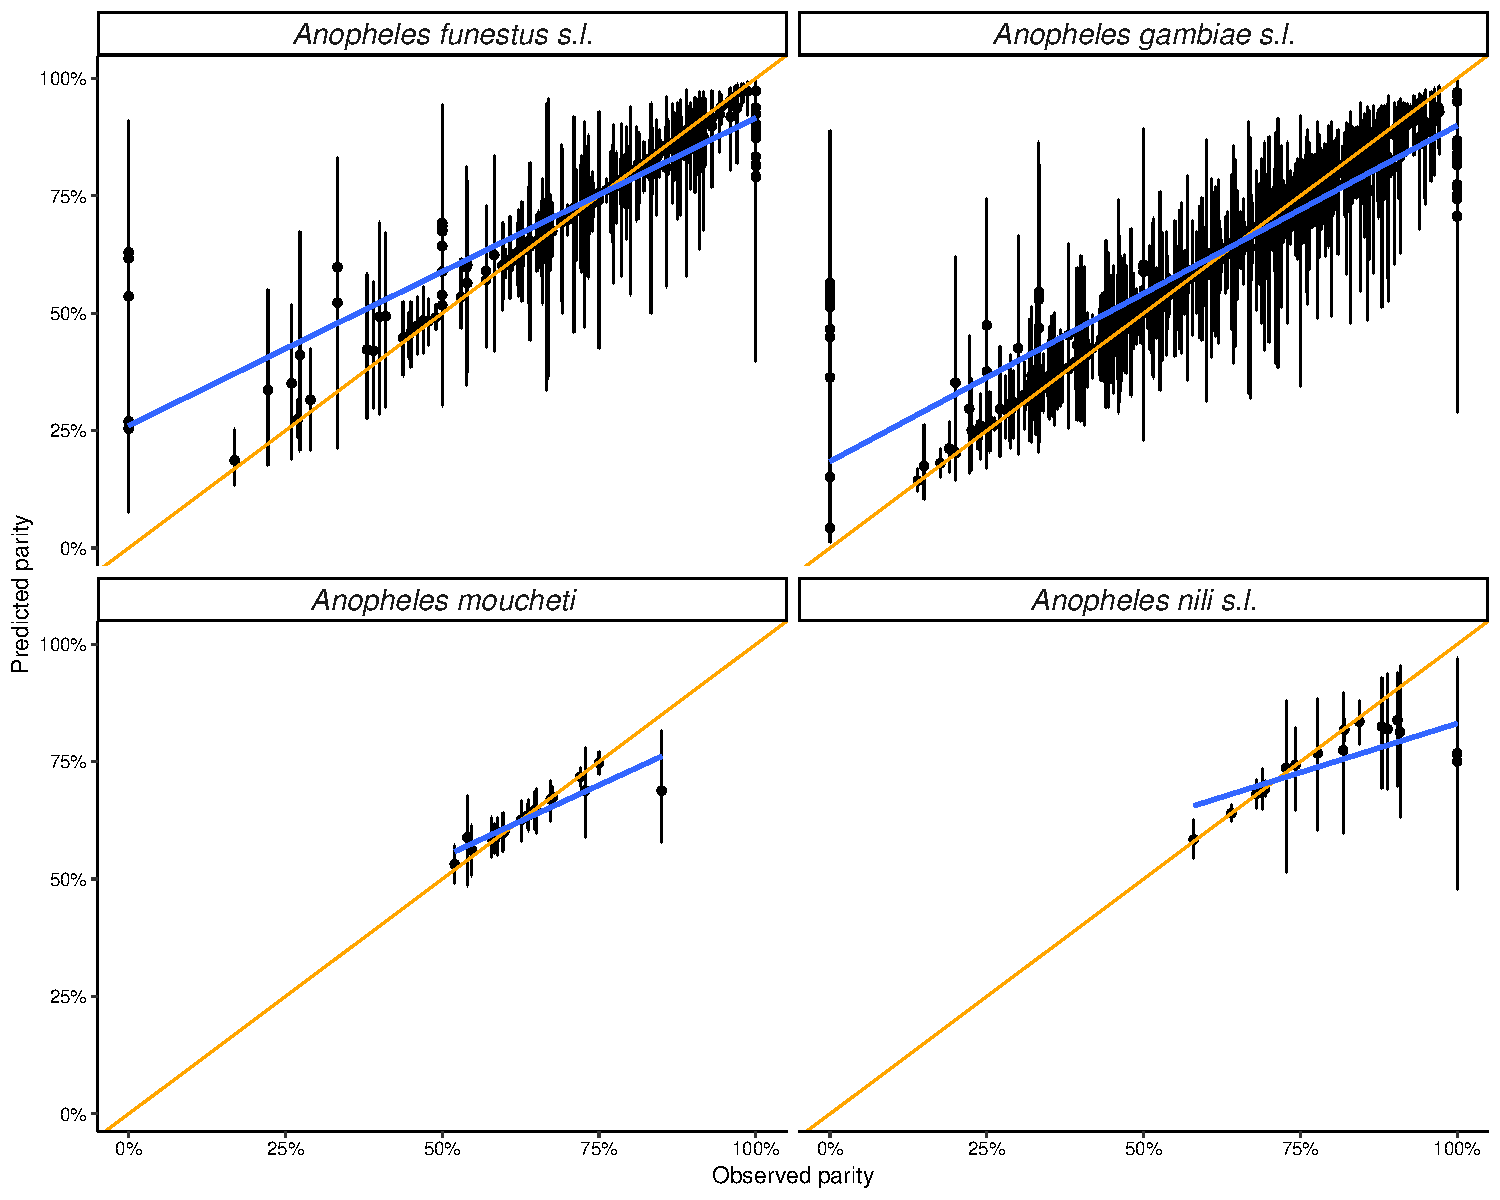
\includegraphics[width=1\textwidth]{./Figure_files/detinova_ppc_africa_grouped.pdf}}
	\caption{\textbf{Posterior predicted parity versus observed quantities for African anopheline samples at the complex level.} The upper and lower extent of the vertical error bars indicate 97.5\% and 2.5\% credible intervals and points indicate posterior medians. The blue lines show linear models fitted to pairs of posterior medians and observed parities, and orange ones show the ${\text{observed}=\text{predicted}}$ line. The analysis was run using 200 iterations per chain across 4 chains, with 100 of the initial samples discarded as warm-up.}\label{fig:detinova_ppcs_africa_grouped}
\end{figure}

\begin{figure}[ht]
	\centerline{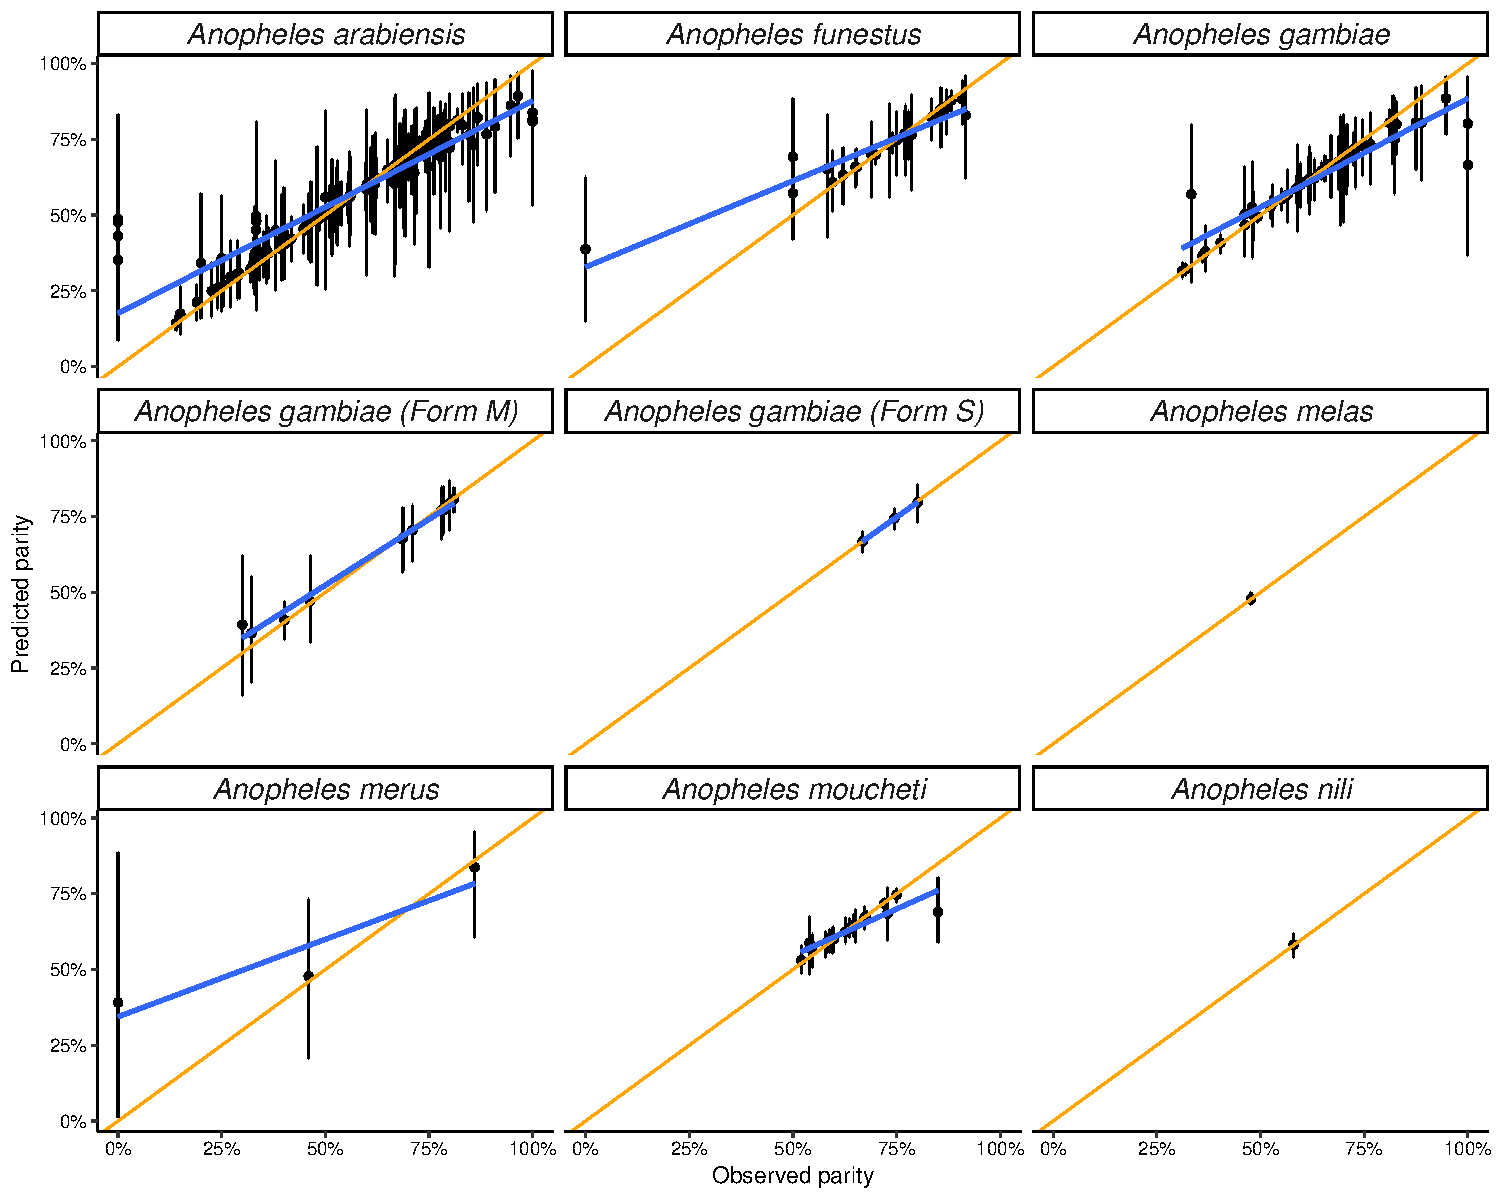
\includegraphics[width=1\textwidth]{./Figure_files/detinova_ppc_africa_species.pdf}}
	\caption{\textbf{Posterior predicted parity versus observed quantities for African anopheline samples at the species level.} The upper and lower extent of the vertical error bars indicate 97.5\% and 2.5\% credible intervals and points indicate posterior medians. The blue lines show linear models fitted to pairs of posterior medians and observed parities, and orange ones show the ${\text{observed}=\text{predicted}}$ line. The analysis was run using 200 iterations per chain across 4 chains, with 100 of the initial samples discarded as warm-up.}\label{fig:detinova_ppcs_africa_species}
\end{figure}

\begin{figure}[ht]
	\centerline{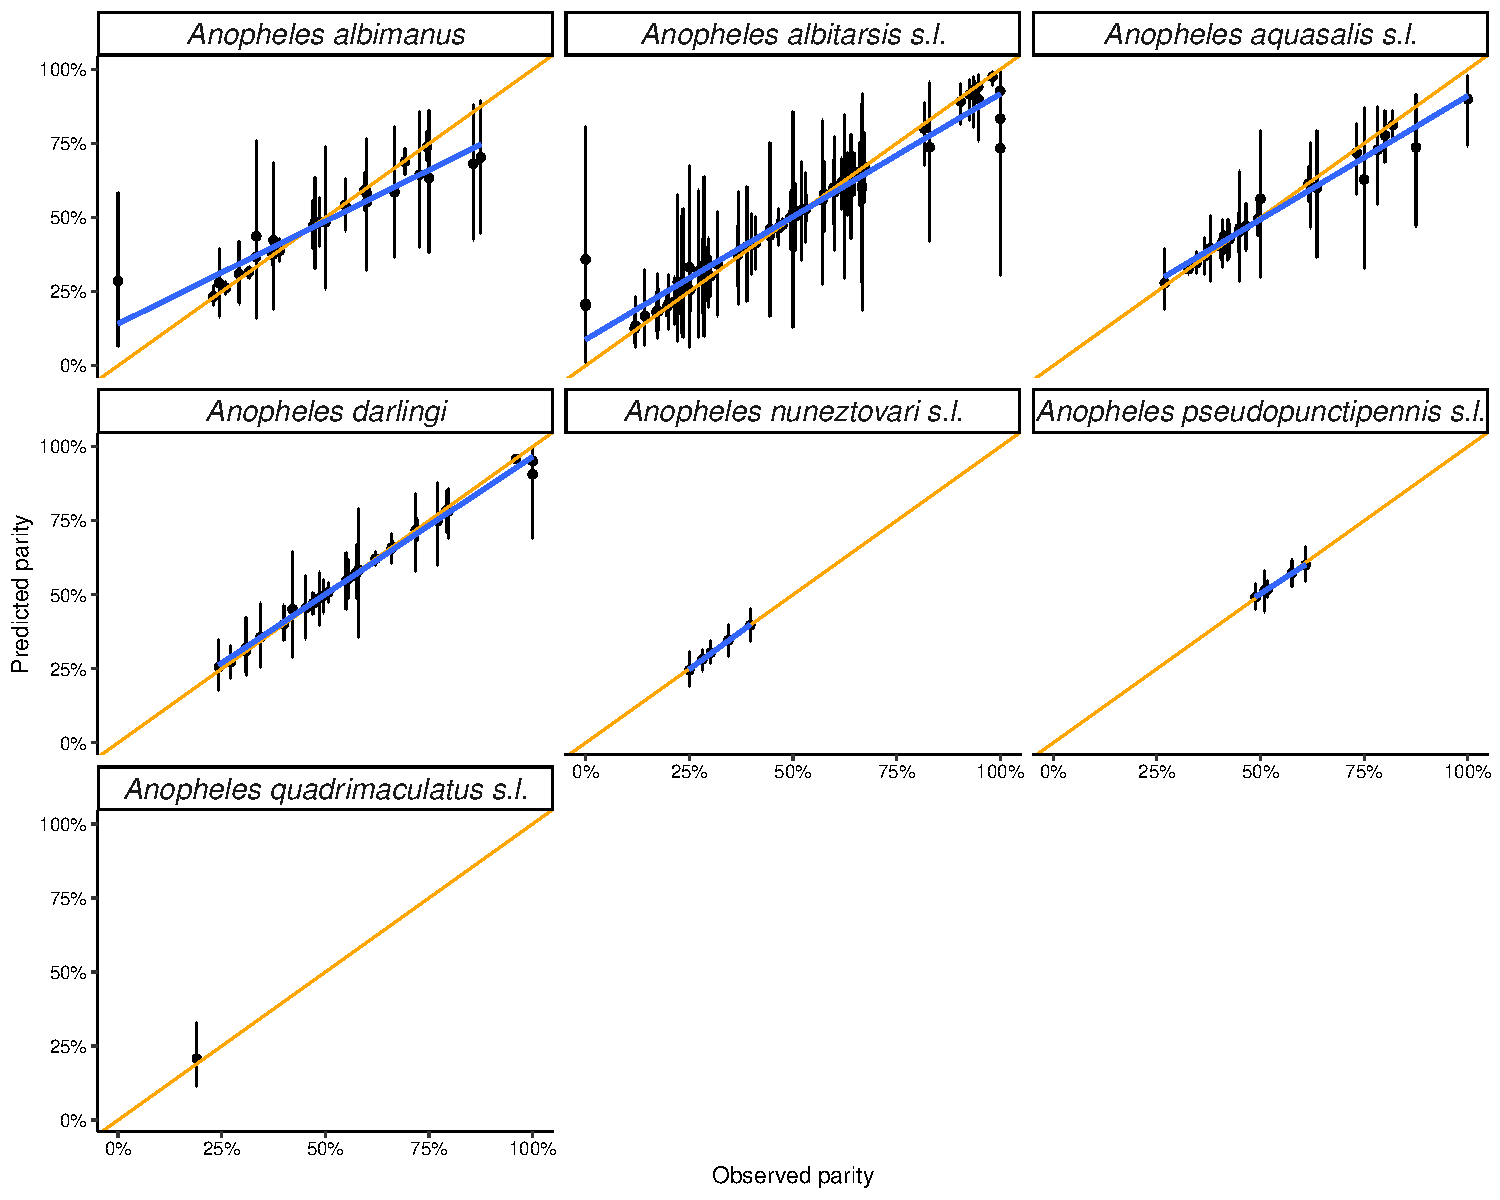
\includegraphics[width=1\textwidth]{./Figure_files/detinova_ppc_americas_grouped.pdf}}
	\caption{\textbf{Posterior predicted parity versus observed quantities for American anopheline samples at the complex level.} The upper and lower extent of the vertical error bars indicate 97.5\% and 2.5\% credible intervals and points indicate posterior medians. The blue lines show linear models fitted to pairs of posterior medians and observed parities, and orange ones show the ${\text{observed}=\text{predicted}}$ line. The analysis was run using 200 iterations per chain across 4 chains, with 100 of the initial samples discarded as warm-up.}\label{fig:detinova_ppcs_americas_grouped}
\end{figure}

\begin{figure}[ht]
	\centerline{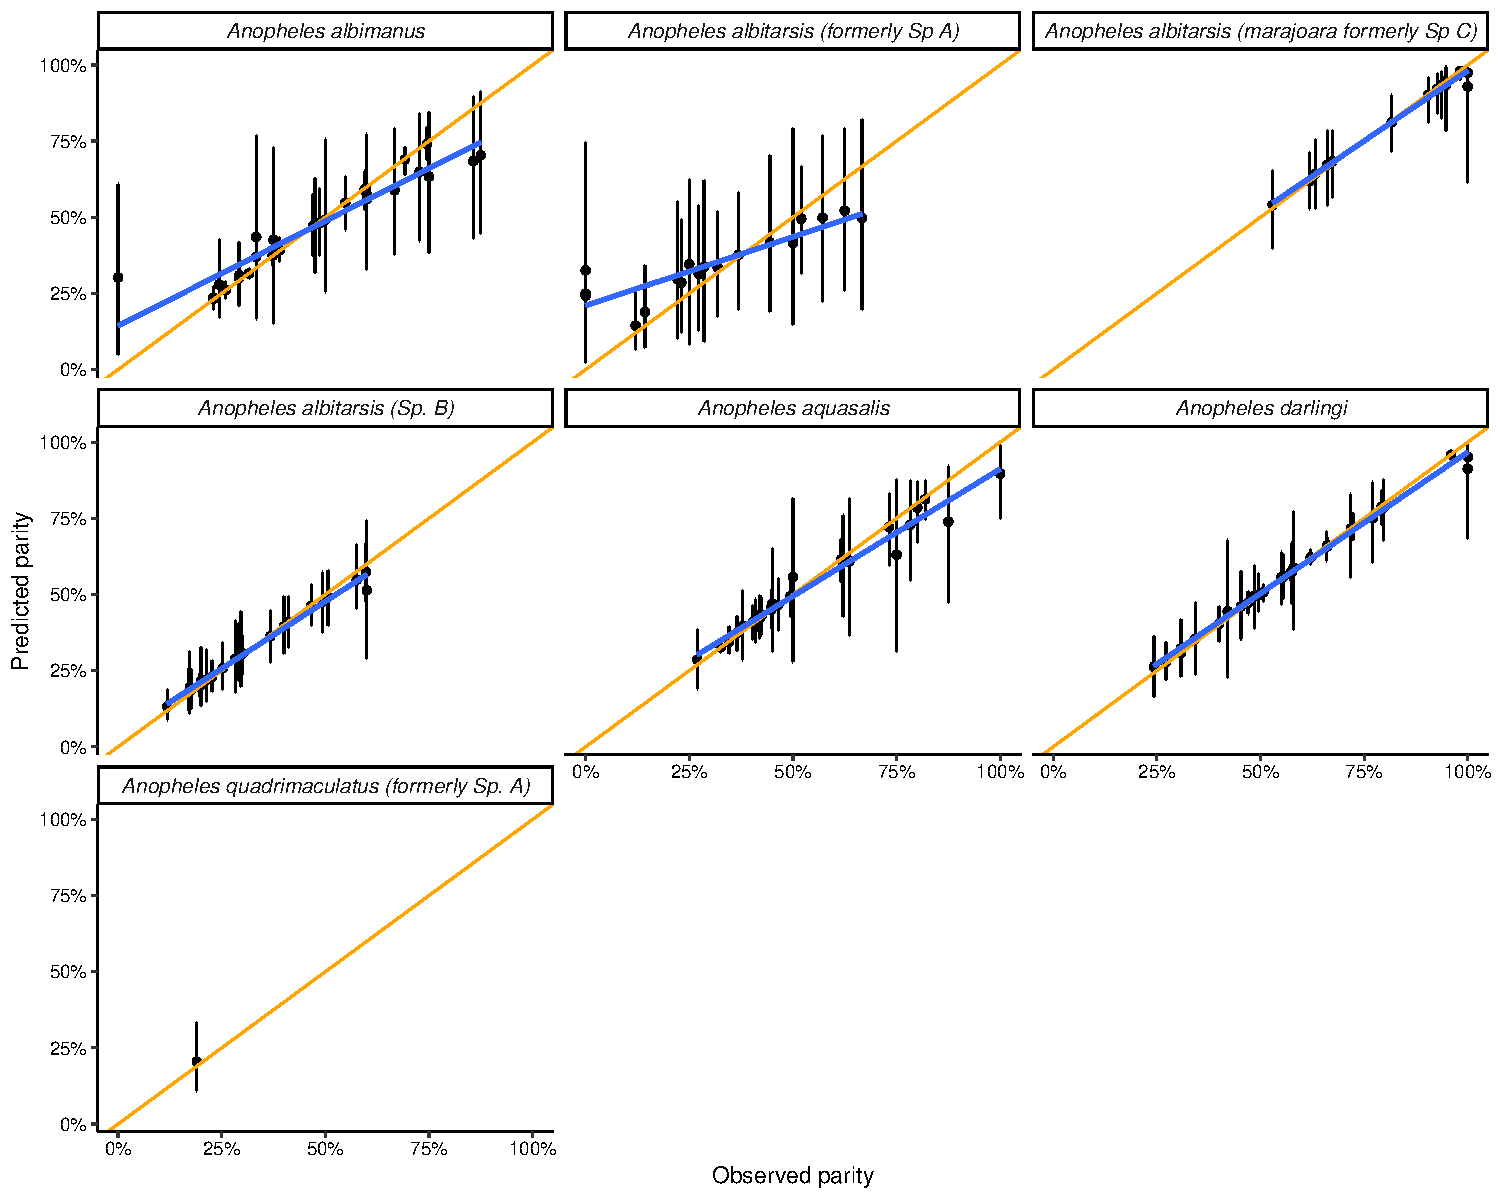
\includegraphics[width=1\textwidth]{./Figure_files/detinova_ppc_americas_species.pdf}}
	\caption{\textbf{Posterior predicted parity versus observed quantities for American anopheline samples at the species level.} The upper and lower extent of the vertical error bars indicate 97.5\% and 2.5\% credible intervals and points indicate posterior medians. The blue lines show linear models fitted to pairs of posterior medians and observed parities, and orange ones show the ${\text{observed}=\text{predicted}}$ line. The analysis was run using 200 iterations per chain across 4 chains, with 100 of the initial samples discarded as warm-up.}\label{fig:detinova_ppcs_americas_species}
\end{figure}


\begin{figure}[ht]
	\centerline{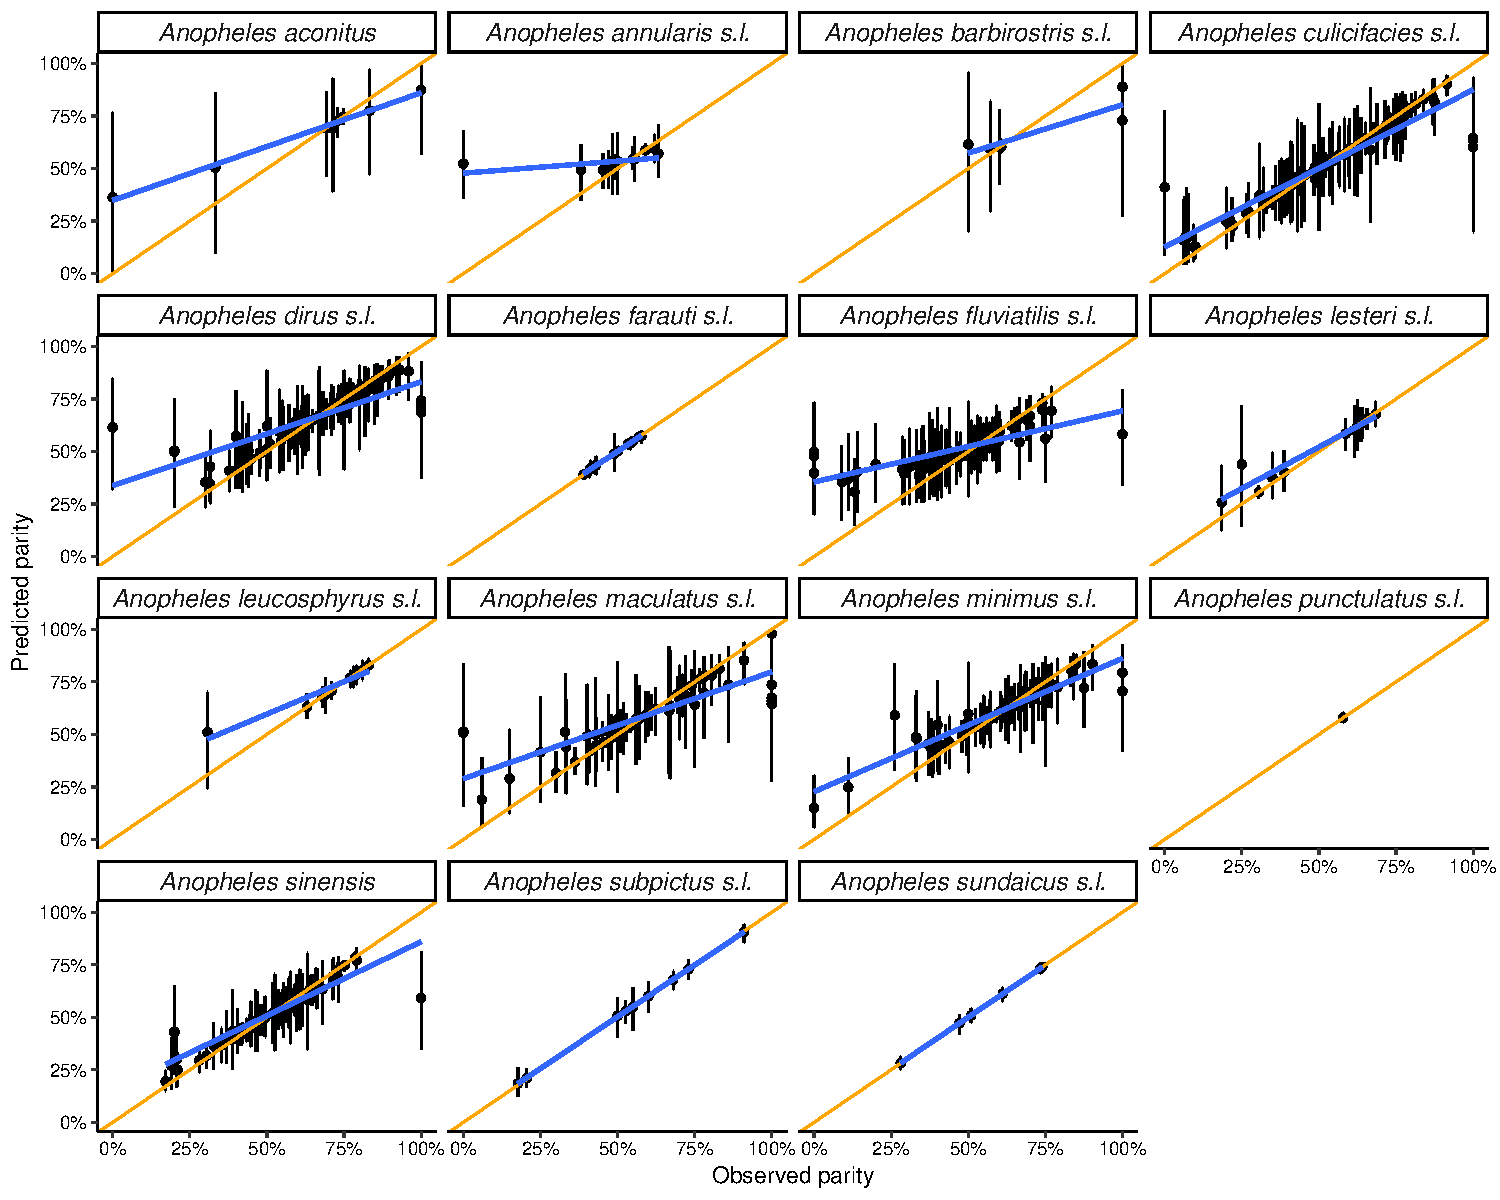
\includegraphics[width=1\textwidth]{./Figure_files/detinova_ppc_asia_grouped.pdf}}
	\caption{\textbf{Posterior predicted parity versus observed quantities for Asian anopheline samples at the complex level.} The upper and lower extent of the vertical error bars indicate 97.5\% and 2.5\% credible intervals and points indicate posterior medians. The blue lines show linear models fitted to pairs of posterior medians and observed parities, and orange ones show the ${\text{observed}=\text{predicted}}$ line. The analysis was run using 200 iterations per chain across 4 chains, with 100 of the initial samples discarded as warm-up.}\label{fig:detinova_ppcs_asia_grouped}
\end{figure}

\begin{figure}[ht]
	\centerline{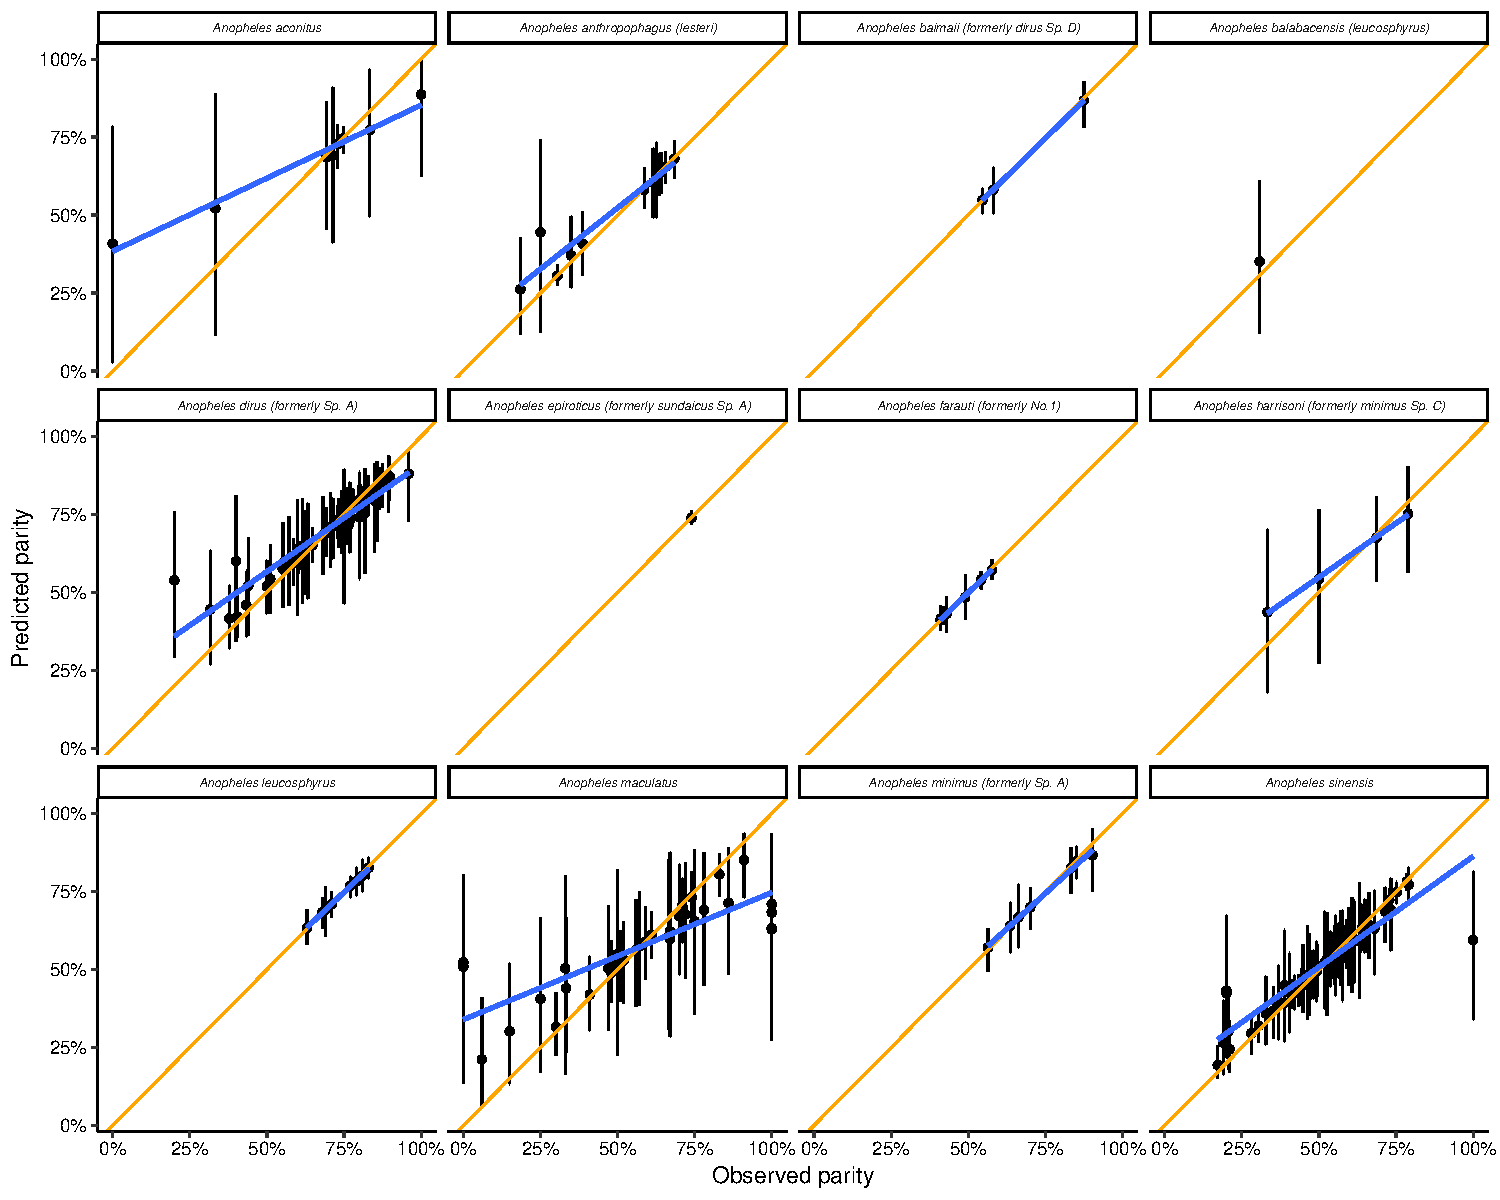
\includegraphics[width=1\textwidth]{./Figure_files/detinova_ppc_asia_species.pdf}}
	\caption{\textbf{Posterior predicted parity versus observed quantities for Asian anopheline samples at the species level.} The upper and lower extent of the vertical error bars indicate 97.5\% and 2.5\% credible intervals and points indicate posterior medians. The blue lines show linear models fitted to pairs of posterior medians and observed parities, and orange ones show the ${\text{observed}=\text{predicted}}$ line. The analysis was run using 200 iterations per chain across 4 chains, with 100 of the initial samples discarded as warm-up.}\label{fig:detinova_ppcs_asia_species}
\end{figure}

\section{EIPs of vector species of malaria, dengue fever, chikungunya and Zika}
The following anopheline species were identified as vector species of malaria,

\begin{itemize}
	\item \textbf{Africa}: \textit{A. gambiae s.l.}, \textit{A. funestus} and \textit{A. melas} \citep{sinka2012global}, and \textit{A. rivulorum} \citep{wilkes1996anopheles}.
	\item \textbf{Americas}: \textit{A. albimanus}, \textit{A. albitarsis}, \textit{A. darlingi}, \textit{A. pseudopunctipennis} and \textit{A. quadrimaculatus} \citep{sinka2012global}; \textit{A. bellator}  \citep{forattini1999role,lorenz2012morphometrical}; \textit{A. cruzii} \citep{lorenz2012morphometrical}; and \textit{A. vestitipennis} \citep{sinka2010dominant}.
	\item \textbf{Europe and the Middle-East}: \textit{A. sergentii} \citep{sinka2012global}; and \textit{A. maculipennis} \citep{hackett1935varieties}.
	\item \textbf{Asia}: \textit{A. farauti s.l.}, \textit{A. koliensis}, \textit{A. lesteri}, \textit{A. maculatus}, \textit{A. minimus}, \textit{A. punctulatus}, \textit{A. stephensi} and \textit{A. subpictus s.l.} \citep{sinka2012global}; and \textit{A. culicifacies} \citep{green1980chromosomal}.
\end{itemize}

For dengue fever, chikungunya and Zika, the main vector species are \textit{Ae. aegypti} and \textit{Ae. albopictus} \citep{kraemer2015global,grard2014zika,benelli2016declining}. 


\section{Studies included in the MRR meta-analysis}\label{sec:appendix_mrrStudyList}
The following is the subset of studies from the original \cite{guerra2014global} database which were used in the MRR meta-analysis: \cite{marini2010study,baber2010population,lacroix2009dispersal,maciel2008calculating,midega2007estimating,maciel2007daily,elizondo2006gonotrophic,ba2005aspects,fabian2005mark,la2004anopheles,watson2000aedes,harrington2001analysis,tsuda2001movement,muir1998aedes,toure1998mark,quinones1997anopheles,costantini1996density,trpis1995estimates,jensen1994comparison,fernandez1994gonotrophic,jaal1992mark,rodriguez1992gonotrophic,chiang1991capture,jensen1991assessment,eldridge1990daily,macdonald1968mark,pumpuni1989population,charlwood1987mark,charlwood1989capture,birley1989effect,arredondo1998gonotrophic,hii1990estimation,renshaw1994host,milby1989estimation,maciel2007body,loong1990survival,nelson1980dispersal,maciel2006movement,mcdonald1977population,curtis1980preliminary,rawlings1982dispersal,conway1974population,reisen1979anopheles,nelson1978estimates,rawlings1981influence,sempala1981ecology,takagi1995movement,buei1980field,eyles1943experiment,ordonez2001use,pant1973field,charlwood1988evidence,reisen1982anopheles,nayar1980quantitative,carnevale1979etude,eyles1946long,reisen1984impact,charlwood1986capture,trpis1975demonstration,lutwama1994mark,wada1969dispersal,takken1998dispersal,abdel1966study,valerio2012dispersal,zetek1915behavior,takagi1995movement,yasuno1975migration,eyles1943measurement,germain1974evaluation}.

\section{Studies included in the dissection study meta-analysis}\label{sec:appendix_dissectionStudyList}
The following is a list of studies included in the dissection study meta-analysis: \cite{catangui1971studies,charlwood1979studies,chang1991comparative,charlwood2000dry,edalat2015vectorial,de2011survivorship,lines1991human,magesa1991trial,lines1991monitoring,forattini1996studies,samarawickrema1967study,samarawickrema1968biting,de2007parity,charlwood1985assessing,chandra1996age,hoc1995ovariole,vythilingam1997abundance,russell1986culex,chadee2010oviposition,ebsary1977biting,charlwood1980observations,shriram2011population,mahmood1981duration,samarawickrema1987seasonal,uttah2013physiological,ramaiah1992non,buei1982age,chadee1995seasonal,chandra2008age,foll1966conditions,kanda1975epidemiological,mala2014gonotrophic,shalaby1962studies,world1960preliminary,reisen1980anopheles,detinova1962age,smith1994age,jayanetti1987study,ch2013comparative,pant1962distribution,ghosh2010seasonal,mahanta1999temporal,schlein2012diurnal,penilla2002pteridine,schlein2015decrease,snow1978host,detinova1968age,nathan1981bancroftian,charlwood1985blood,schlein2008approach,beier2012attractive,muller2005plant,surendran2006anopheles,muller2010successful,mendis1998cordon,wilkes1996anopheles,chatterjee2000role,muller2010successful,tuchinda1969diurnal,chan1971life,aigbodion2011pelagia,qualls2015indoor,reisen1981anopheles,gillies1972range,gillies1965study,kay1979age,hitchcock1968age}.

\section{Studies included in the gonotrophic cycle duration meta-analysis}\label{sec:appendix_gonotrophicDurationStudyList}
The following is a list of studies included in the gonotrophic study meta-analysis: \cite{gillies1965study,sheppard1969dynamics,de1967time,pant1973field,germain1974evaluation,lowe1973reproductive,fernandez1994gonotrophic,buei1980field,rawlings1982tests,mori1977gonotrophic,sempala1981ecology,reisen1983population,birley1989effect,suzuki1978preliminary,charlwood1987mark,charlwood1986capture,charlwood1979studies,charlwood1995rise,chang1991comparative,edalat2015vectorial,de2011survivorship,samarawickrema1968biting,samarawickrema1967study,charlwood1985assessing,chandra1996age,russell1986culex,chadee2010oviposition,mahmood1981duration,ahumada2004modeling,kenawy1991development,rajagopalan1980population,chandra2008age,scholl1979aedes,mala2014gonotrophic,afrane2005effects,gillies1953duration,quinones1997anopheles,rua2005laboratory,delatte2009influence,arredondo1998gonotrophic,wong2014sampling,ijumba2002malaria}.



 \bibliographystyle{authordate1}
 \bibliography{Malaria}
\newpage

\end{document}